\documentclass{article}
\usepackage[portuges]{babel}
\usepackage[utf8]{inputenc}
\usepackage[T1]{fontenc}
\usepackage{graphicx}

\usepackage{cite}
\usepackage{float}
\usepackage{enumerate}
\usepackage{makeidx}
\usepackage{booktabs}
\usepackage{pdfpages}
\usepackage{a4wide}
\usepackage{indentfirst}
\usepackage{marvosym}
\usepackage{url}

\setlength\oddsidemargin{0.3in}
\setlength\evensidemargin{-0.3in}
\setlength\headsep{15pt}
\setlength\footskip{30pt} 


% environment created for organization purposes, only.
\newenvironment{TODO}{%
  \color{blue} \itshape \begin{itemize}
}{%
  \end{itemize}
}
%---------------------------------------

% our addimage command
\newcommand{\addimg}[1]{%
  \begin{center}
    \includegraphics[width=0.75\textwidth]{#1}
  \end{center}
}

\newcommand{\RowStretch}[1]{\renewcommand{\arraystretch}{#1}}



%----------------------------------------------------------

\begin{document}


\includepdf[pages=-]{capa}

\tableofcontents
\newpage
\section{Visão Geral do Produto}
  \subsection{Propósito do Produto}
    \subsubsection{Descrição do Problema}

      Hoje em dia, existe uma grande diversidade de atrações e formas de motivar crianças e jovens a gastar dinheiro. Quer lojas físicas, quer virtuais, são cada vez mais acessíveis nos seus métodos de pagamento, e a oferta destes também cresce. Contudo, de uma forma geral, estas faixas etárias estão dependentes do dinheiro que recebem de pais, tutores ou familiares.

      O dinheiro chega, habitualmente, às mãos dos jovens sob a forma de semanadas, mesadas ou ofertas de familiares. É uma oportunidade de lhes transmitir algumas noções sobre o dinheiro e a importância da gestão dele. Mas, numa realidade em que o dia-a-dia é stressante e agitado, nem sempre é fácil os pais se manterem coerentes nas semanadas.

      Apesar de as novas tecnologias facilitarem a comunicação e nos darem algumas comodidades no uso e gestão do dinheiro pessoal, muitos pais ainda recorrem a métodos ineficazes para acompanhamento da educação monetária dos filhos, tornando a experiência custosa. Como agravante, a seleção de tecnologias para disponibilização de dinheiro à distância e controlo de gastos ainda é algo limitada. Assim, torna-se difícil os pais poderem saber quanto dinheiro os seus filhos têm, quanto gastam, e como o gastam.

    \subsubsection{Proposta de Solução}

      A yWallet, o produto descrito neste documento, é um sistema de informação para pagamentos móveis, recorrendo ao Bitcoin como moeda de transação, e oferece uma camada de controlo parental. Essencialmente, permite aos pais controlarem, a qualquer momento e em qualquer lugar, o dinheiro que disponibilizam aos filhos, os gastos destes, e dinheiro que estes recebem de outras fontes, como familiares ou amigos. Inclui uma componente pedagógica que transmite ao jovem algumas dicas práticas para a gestão do seu capital, e oferece filtragem de despesas por categoria ou período, para que todos os utilizadores tenham uma melhor noção de onde e como se está a usar o dinheiro. A camada de controlo parental deve incorporar uma camada de autorização de transações, por exemplo com base na geolocalização do utilizador.

      A visão para esta solução assenta em quatro componentes, com propósitos muito bem definidos. A Figura \ref{img1} ilustra uma possível arquitetura para o produto.

      \begin{figure}[ht!]
        \centering
          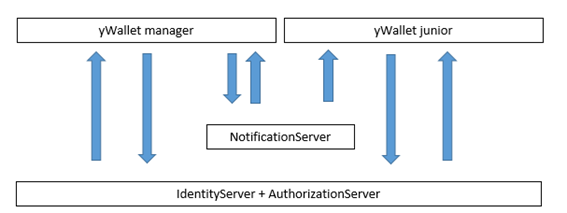
\includegraphics[width=0.7\linewidth]{img/img1}
          \caption{Arquitetura da solução proposta}
          \label{img1}
      \end{figure}

      No nível aplicacional, com o qual os clientes finais interagem diretamente, temos duas aplicações, a \emph{yWallet Junior} e a \emph{yWallet Manager}. Ambas desenvolvidas para ambientes móveis, e ainda para um contexto web, no caso da \emph{yWallet Manager}. A aplicação \emph{Junior} deverá responder às necessidades de pagamentos móveis por parte dos jovens. Inclui funcionalidades básicas de gestão de conta, como consulta de movimentos e objetivos de poupança. Por outro lado, a aplicação \emph{Manager} permite fazer toda a gestão e/ou acompanhamento detalhado das carteiras dos jovens. É este o componente do sistema responsável pela definição de autorizações de pagamento, regras de controlo parental, ou disponibilização de dinheiro às carteiras \emph{Junior}.

      Os servidores de identidade, autorização e notificação (designados por \emph{Identity Server}, \emph{Authorization Server} e \emph{Notification Server}, respetivamente) visam garantir o cumprimento de vários requisitos relacionados com o processo de gestão/controlo parental, sendo estes parametrizados através do \emph{yWallet Manager} e dos quais o \emph{yWallet Junior} depende. Estes servidores disponibilizam uma camada de serviços, assente em tecnologias REST, que visa facilitar a comunicação entre as suas instâncias e as aplicações cliente. O \emph{Identity Server} é a camada do sistema que lida com o acesso às contas dos utilizadores, enquanto o \emph{Authorization Server} resolve o problema de autorizações para as diversas operações. Por fim, o \emph{Notification Server} permite o envio de notificações \emph{push} para os clientes móveis.

  \subsection{Clientes e Stakeholders}
    \subsubsection{Clientes}
      O principal propósito desta aplicação é ajudar o jovem a fazer a gestão da sua mesada/semanada. No entanto, a aplicação só funciona quando existem duas partes. Assim sendo, o público-alvo da nossa aplicação são tanto os jovens que dependem dos pais para obter dinheiro, como os próprios pais, pois esta interliga e traz vantagens para ambas as partes. Torna-se então importante fazer uma análise da demografia do mercado referente a estas diferentes faixas etárias.

      Numa primeira abordagem, vemos que estas se tratam de gerações distintas com aptidões e vontades diferentes. Estas gerações estão catalogadas nas teorias demográficas e há uma interseção de gerações dos pais dos filhos a quem a nossa aplicação é destinada. Essas duas gerações são conhecidas como \emph{Baby-Boomers} e \emph{Geração X}. A geração dos Baby-Boomers alberga todos os pais com 50 e mais anos, enquanto a Gen X engloba os pais nascidos entre 1965 e 1975. Os baby-boomers são conhecidos por ter grande poder económico e, por ano, gastam mais de 400 mil milhões de dólares que qualquer outra geração. É importante também saber que têm um \emph{Complexo de Peter Pan}, e não gostam de se sentir velhos e ultrapassados. Os pais incluídos na geração X estão agora, de uma forma geral, em topo de carreira, quando ganham e gastam mais, mas também têm grande interesse na poupança. Dão grande importância à educação e ao conhecimento, e são experientes na tecnologia.

      A \emph{Geração Y}, a geração dos filhos, tem as suas idades compreendidas entre os 9 e os 27 anos. Tendo crescido lado a lado com a tecnologia, esta geração é particularmente responsiva a campanhas na Internet. Processam a informação muito rapidamente e são fiéis às marcas. Respondem bem a marketing inovador, bem-humorado e ``outside the box''.

      Todos estes fatores são relevantes, quando se está a criar um produto direcionado a diferentes faixas etárias. Mais ainda, estudos revelam que no final deste ano é esperado que 1,76 mil milhões de pessoas no mundo possuam smartphones (Smartphone Users Worldwide Will Total 1.75 Billion, 2015). Restringindo-nos a estudos realizados nos Estados Unidos da América (Press Releases - 2014 Digital Wallet Usage Study, 2014), para levar a cabo uma análise de como seria recebido o nosso produto, sabemos que 80\% da população americana tem conhecimento do que são carteiras digitais, 32\% dessas pessoas já as utilizou para realizar compras, e 43\% dessas compras foram feitas por pessoas situadas na faixa etária dos 18 aos 29 anos, sendo esta a faixa etária predominante na utilização deste método de pagamento.

    \subsubsection{Stakeholders}  

      Os stakeholders do projeto são todas as partes interessadas ou intervenientes ao longo do ciclo de vida do projeto, e que podem gerar requisitos para o projeto. Os principais stakeholders deste projeto são:

        \begin{description}
          \item[Group Buddies,]a empresa que propôs o tema deste projeto;
          \item[Equipa docente da unidade curricular Projeto de Engenharia Informática,] que acompanha o desenvolvimento do projeto e avaliará o desempenho da equipa e o produto final;
          \item[Equipa do Projeto,] responsável pelo planeamento e realização do projeto e pela produção da documentação;
          \item[Pais com filhos economicamente dependentes,]que terão interesse em adquirir o produto, que os ajudará a gerir o dinheiro dos seus filhos;
          \item[Jovens economicamente dependentes,] os utilizadores finais do produto, com o qual poderão receber dinheiro dos pais e efetuar as compras no seu dia-a-dia.
        \end{description}

      Note-se que por pais com filhos economicamente dependentes designam-se as pessoas que suportem algum jovem economicamente, seja esse jovem filho ou não.

  \subsection{Utilizadores do Produto}

    No desenvolvimento de um sistema de informação é crucial determinar os perfis de utilização, ou classes de utilizadores, do sistema. Estes permitem não só identificar os casos de uso esperados, como ajudam a garantir que os requisitos especificados respondem às necessidades de cada tipo de utilizador.

    \subsubsection{Pai}

      \begin{description}
        \item[Categoria] Utilizador Principal
        \item[Experiência na matéria] Qualquer. Esta classe engloba utilizadores com muita, pouca ou nenhuma experiência em gestão do dinheiro de jovens monetariamente dependentes.
        \item[Experiência tecnológica] Razoável. Esta classe engloba utilizadores com muita ou pouca experiência tecnológica. Utilizadores sem experiência tecnológica terão uma tendência natural para não procurar ou entender este produto, dado o uso de meios eletrónicos de pagamento e transferência de dinheiro. Estes utilizadores podem ter menos experiência com smartphones do que com computadores.
        \item[Descrição] Os pais disponibilizam dinheiro aos filhos e podem definir regras que os filhos terão que respeitar ao utilizar o dinheiro. Podem também ver estatísticas da utilização do dinheiro dos filhos.
        Os pais podem ser vistos como utilizadores menos ativos da aplicação, uma vez que a sua principal obrigação é fornecer dinheiro aos jovens. No entanto, este pode ter um papel mais ativo conforme ache necessário.
        \item[Participação no sistema] Diária ou muito frequente. É esperado que este utilizador interaja com a aplicação em consultas rápidas, algumas vezes ao dia, ou em intervalos de alguns dias. Ocasionalmente poderá ter períodos de uso mais longos, por exemplo para aplicar ações de controlo parental. Estes utilizadores contribuirão para o produto produzindo requisitos de usabilidade, fornecendo feedback geral sobre o produto, reportando erros e partilhando conhecimento na matéria de gestão de dinheiro de jovens.
      \end{description}

    \subsubsection{Jovem}

      \begin{description}
        \item[Categoria] Utilizador Principal
        \item[Experiência na matéria] Qualquer. Esta classe engloba utilizadores com muita, pouca ou nenhuma experiência em gestão pessoal de dinheiro e pagamentos eletrónicos.
        \item[Experiência tecnológica] Razoável. Esta classe engloba utilizadores com muita ou pouca experiência tecnológica. É expectável alguma experiência com smartphones, aplicações móveis e computadores.
        \item[Descrição] Os jovens serão os principais utilizadores da aplicação, através da qual irão efetuar pagamentos, podendo também definir as suas próprias regras para melhor gerirem o seu dinheiro. Se apresentarem comportamentos menos responsáveis poderão receber avisos que os sensibilizarão a praticar outros hábitos. Terão também a possibilidade de, em caso de necessidade, pedir mais dinheiro aos pais.
        \item[Participação no sistema] Diária. Estes utilizadores farão uso do produto no seu dia-a-dia, possivelmente várias vezes num mesmo dia para consultas de conta ou efetuar pagamentos. Estes utilizadores contribuirão para o produto produzindo requisitos de usabilidade, fornecendo feedback geral sobre o produto e reportando erros.
      \end{description}

    \subsubsection{Desenvolvedor}

      \begin{description}
        \item[Categoria] Técnicos de Serviço e Manutenção
        \item[Experiência na matéria] Razoável. Os utilizadores desta classe podem não ter necessariamente experiência em gerir dinheiro de jovens monetariamente dependentes, mas têm um conhecimento suficiente da matéria, através de estudo, para entenderem as necessidades dos outros utilizadores.
        \item[Experiência tecnológica] Experiente. As tecnologias, sejam computadores, smartphones, ou outros, fazem parte do dia-a-dia desta classe de utilizador.
        \item[Descrição] Os utilizadores desta classe são responsáveis pela produção, manutenção e garantia de qualidade do produto.
        \item[Participação no sistema] Muito frequente. Este utilizador contribui para o sistema, desde o seu desenvolvimento, em várias tarefas, como modelação, prototipagem e teste. Depois de lançado o produto, é responsável por resolver eventuais problemas reportados pelos outros utilizadores, e desenvolver novas versões do produto.
      \end{description}

    \subsubsection{Administrador}

      \begin{description}
        \item[Categoria]Técnicos de Serviço e Manutenção.
        \item[Experiência na matéria]Razoável. Os utilizadores desta classe podem não ter necessariamente experiência em gerir dinheiro de jovens monetariamente dependentes, mas têm um conhecimento suficiente da matéria, através de estudo, para entenderem as necessidades dos outros utilizadores.
        \item[Experiência tecnológica]Experiente. As tecnologias, sejam computadores, smartphones, ou outros, fazem parte do dia-a-dia desta classe de utilizador.
        \item[Descrição]Os administradores são responsáveis por gerir as contas dos utilizadores, procurando possíveis anomalias ou infrações. Serão também responsáveis por administrar a infraestrutura do sistema.
        \item[Participação no sistema]Diária. Este utilizador contribui para o sistema com diversas tarefas administrativas, e respondendo a pedidos de suporte de outros utilizadores.   
      \end{description}

  \subsection{Concorrentes}

    Apesar da oferta de tecnologias para controlo de dinheiro e gastos de jovens ser reduzida, existem alguns concorrentes no mercado a ter em consideração. Uma parte considerável destes concorrentes aposta em cartões de débito pré-pagos, oferecendo as comodidades de um cartão, e mantendo as restrições de gastos.

    \subsubsection{Escolas}

      Já é habitual as escolas disponibilizarem um cartão de estudante que serve também de cartão de débito pré-pago no interior da escola.

      \begin{description}
        \item[Funcionalidades] Este método oferece ao jovem as comodidades de efetuar pagamentos com cartão, e oferece aos pais um método simples de controlo de despesas, com maior ou menor granularidade, dependendo do sistema implementado.

        \item[Limitações] Os cartões escolares estão restritos a uso escolar, e, portanto, não contribuem para gestão de despesas para além deste contexto.
      \end{description}


    \subsubsection{Cartão LOL da Caixa Geral de Depósitos}

      Alguns bancos, como a Caixa Geral de Depósitos, oferecem cartões de débito pré-pagos para menores.

      \begin{description}
        \item[Funcionalidades] Permite ao jovem efetuar pagamentos com cartão, de forma semelhante a um cartão habitual, e permite aos pais controlarem as transações e os carregamentos. Opcionalmente o jovem pode aplicar um plano de poupança.
        \item[Limitações]Impõe comissões de carregamento do cartão.
      \end{description}


    \subsubsection{Allowance Manager}

      Allowance Manager é uma aplicação com o propósito de ajudar os pais a introduzirem crianças a uma gestão autónoma do seu dinheiro.

      \begin{description}
        \item[Funcionalidades]Oferece uma aplicação para os pais gerirem e controlarem contas dos filhos. Permite notificações por mensagem quando ocorrem transações. Auxilia na automatização das semanadas. Na sua versão paga, é disponibilizado um cartão de débito pré-pago, para que a criança possa interagir e aprender a gerir dinheiro real.
        \item[Limitações]Apenas a versão paga permite fazer pagamentos. A versão gratuíta só permite fazer o registo manual das transações.
        \item[Concorrentes semelhantes]Osper
      \end{description}
      
    \subsubsection{Simple}

      O simple é um serviço bancário pessoal.

      \begin{description}
        \item[Funcionalidades]Oferece um cartão Visa para efetuar pagamentos. Oferece uma aplicação para gestão da conta pessoal, com visão detalhada sobre despesas, planos de poupança e permite ainda transferências imediatas entre utilizadores.
        \item[Limitações]Apesar da qualidade do serviço, não oferece uma alternativa com controlo parental para jovens.
      \end{description}
      
    \subsubsection{Carteiras Digitais}  

      A crescente vaga de carteiras digitais facilita pagamentos com tecnologias alternativas a cartões, baseadas em smartphones.

      \begin{description}
        \item[Funcionalidades]Oferecem contas com associação a cartões, de forma a realizar pagamentos por meios eletrónicos, sem cartão ou dinheiro físico. Suportam tecnologias como pagamentos por SMS, leitura de códigos QR, ou protocolos NFC. Permitem também a visualização do histórico de transações, e transferências instantaneas entre utilizadores.
        \item[Limitações]Não oferecem uma vertente de controlo parental para os jovens.
      \end{description}

  \subsection{Oportunidade e Modelo de Negócio}

    Assim surge a nossa oportunidade de negócio a partir da necessidade que os pais têm de controlar e gerir os gastos dos filhos, assim como da necessidade que os filhos têm de receber dinheiro dos pais e saber como gerí-lo durante determinado período de tempo.

    Nenhum dos concorrentes existentes oferecem o que estamos a propor: Uma aplicação que permite fazer transferências (\emph{yWallet Manager }para \emph{yWallet Junior}) e pagamentos e, ao mesmo tempo gerir e controlar o dinheiro que resta, tanto por parte do filho como do pai. Como a moeda utilizada será o Bitcoin, todas as transfências de dinheiro serão instantâneas e livres de custos, tanto entre pai e filho como os próprios pagamentos (o que adiciona valor para os vendedores).
  
    No entanto, sendo este um negócio, é necessário um modelo de negócios adequado para que o produto possa ser rentável. Para isso, irá ser utilizado o modelo de negócios \emph{freemium}.
  
    A aplicação \emph{yWallet manager} permitirá associar uma ou mais contas \emph{yWallet junior}, sendo que estas por sua vez poderão ser contas \emph{Free} ou \emph{Premium}. As contas \emph{Free}, como o próprio nome indica não vão gerar receitas, e servirão apenas de forma divulgar a aplicação e eventualmente ajudar a cativar clientes \emph{Premium}. Os utilizadores com contas \emph{Free} só terão acesso às funcionalidades mais básicas da aplicação. As contas \emph{Premium} vão ver a fonte de receitas da solução proposta, sendo estas as que vão permitir gerar negócio. Os cliente com contas deste tipo terão acesso a todas as funcionalidades da aplicação. Para mais detalhes, consultar o documento anexo ``Plano de Negócios''.

\newpage

\section{Restrições do Projeto}
  
  \subsection{Mandated Constraints}

    A realização de um projeto de software pode estar afetada por restrições de várias naturezas, imposições difíceis ou impossíveis de contornar na prática. Podemos afirmar que o produto estará assente em tecnologia existente e testada, largamente usada pelo público em geral. Não será necessário inventar uma nova tecnologia para a concretização deste produto. De um modo geral, a maioria das restrições aplicáveis a este produto são sociais, orçamentais ou temporais, em vez de restrições técnicas.

    \subsubsection{Restrições da Solução}

      \begin{description}
        \item[Descrição]O produto deve comunicar com o servidor, por HTTPS com recurso a \emph{certificate pinning}.
        \item[Fundamentação]O produto deve comunicar por HTTPS com recurso a \emph{certificate pinning} para aumentar a sua segurança e para evitar ataques \emph{man-in-the-middle}.
        \item[Critério de validação]Toda a comunicação entre a aplicação e o servidor deve ser cifrada e não deve ser possível alguém intercetar a comunicação e decifrar a mesma.
      \end{description}

\vspace{0.7cm}

      \begin{description}
        \item[Descrição]A aplicação resultante deve executar num smartphone.
        \item[Fundamentação]O produto final deve integrar uma aplicação móvel, permitindo ser transportado para onde o utilizador tiver que efetuar pagamentos.
        \item[Critério de validação]O produto deve poder ser instalado num smartphone Android, Windows Phone 8, ou iPhone.
      \end{description}
\vspace{0.7cm}

      \begin{description}
        \item[Descrição]O produto deve permitir trabalhar em modo offline.
        \item[Fundamentação]O produto deve permitir a consulta de operações históricas já realizadas no dispositivo mesmo que este não possua acesso à rede, e sincronizar assim que esteja novamente conetado, por forma a não limitar o utilizador a utilizar a aplicação apenas quando tiver acesso à Internet.
        \item[Critério de validação]O produto deve permitir a consulta de operações históricas já realizadas no dispositivo mesmo que este não possua acesso à rede.
      \end{description}

\vspace{0.7cm}
      \begin{description}
        \item[Descrição]A aplicação deve usar WebSockets para comunicação bidirecional.
        \item[Fundamentação]A aplicação deve usar WebSockets para comunicação bidirecional e tempo quase real, permitindo assim receber mensagens do servidor, tais como pedidos de autorização de pagamento.
        \item[Critério de validação]A aplicação deve ser capaz de fazer pedidos ao servidor assim como responder a pedidos feitos pelo servidor.
      \end{description}


    \subsubsection{Ambiente de Implementação do Sistema Atual}

      O ambiente onde a aplicação vai ser utilizada não se restringe a nenhum local físico, e, quando ligada à Internet, deve proporcionar comunicação com os servidores de identidade e autorização, assim como estar acessível a partir do servidor de mensagens push.

      \begin{figure}[ht!]
        \centering
          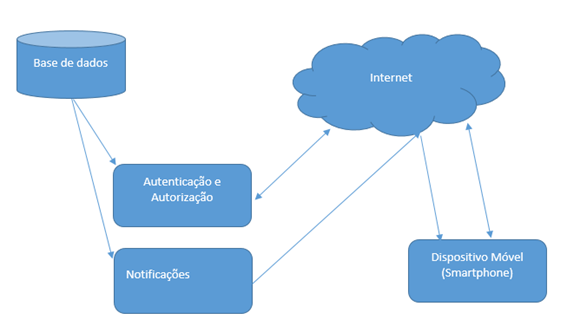
\includegraphics[width=0.7\linewidth]{img/img2}
          \caption{Ambiente de Implementação}
          \label{img2}
      \end{figure}

    \subsubsection{Parceiros ou Aplicações Colaborativas}

      \begin{description}
        \item[Descrição]O produto deve recorrer à API do Bitreserve ou do Coinbase.
        \item[Fundamentação]Estas API foram sugeridas pelos stakeholders. O produto deve usar uma destas API para garantir a não volatilidade da moeda aos clientes, assim como assegurar a transparência das transações. Adicionalmente, o uso destas API servirá para colmatar o tempo de espera nas confirmações de pagamento, assim como para eliminar ou minimizar custos de conversão de moeda.
        \item[Critério de validação]A aplicação deve ser capaz de realizar as mesmas operações que aquelas disponibilizadas pela API usada, expondo-as para o cliente.
      \end{description}

    \subsubsection{Outras Restrições}  
      \begin{description}
        \item[Descrição]Um protótipo do produto, conforme descrito neste documento, deverá estar pronto em Fevereiro de 2015.

        \item[Tipo de Restrição]Restrição de Planeamento
        \item[Fundamentação]Este produto está a ser desenvolvido no contexto da UCE15 do Mestrado de Engenharia Informática, que decorre no primeiro semestre do ano letivo de 2014/2015, e portanto é imperativo que esteja concluído durante o mês de Fevereiro de 2015.
      \end{description}
\vspace{0.5cm}
      \begin{description}
        \item[Descrição]O produto não deve acarretar custos extraordinários de implementação.
        \item[Tipo de Restrição]Restrição Orçamental

        \item[Fundamentação]O produto não deve acarretar custos de implementação, outros que não as horas de trabalho a ele dedicadas pelos seu desenvolvedores, e deve ser implementável por uma equipa de 9 pessoas durante um período de desenvolvimento de dois meses (Dezembro de 2014 e Janeiro de 2015), considerando uma disponibilidade média de 20 horas semanais por cada elemento.
      \end{description}

  \subsection{Definições e Convenções de Nomenclatura}

    Para o documento ser coerente, é necessário utilizar uma terminologia consistente e explícita. Para este efeito, descrevemos nesta secção essa terminologia, enumeramos os termos e acrónimos utilizados, e o respetivo significado. Nesta secção definimos ainda conceitos e sistemas que serão referidos nas secções de \emph{Âmbito de Trabalho} e \emph{Âmbito do Produto}.

    \subsubsection{Glossário}

      \begin{description}
        \item[Aplicação]Programa informático que visa facilitar a realização de uma tarefa no computador ou em outros dispositivos.
        \item[Bitcoin]Moeda baseada em sistemas digitais.
        \item[Browser]Programa informático que permite aceder a páginas da internet.
        \item[Cartão de crédito]Sistema de pagamento que permite ao utilizador pagar serviços e bens com base na promessa que pagará essas dívidas no futuro.

        \item[Cartão de débito]Sistema de pagamento que permite ao utilizador pagar serviços e bens utilizando o dinheiro que possui numa conta que esteja associada.
        \item[Carteira digital]Sistema de gestão de dinheiro baseado em sistemas digitais.
        \item[Controlo Parental]Sistema de gestão de dinheiro baseado em sistemas digitais.
        \item[Feedback]Juízo de valor sobre um serviço ou funcionalidade, com o propósito de aconselhar outras pessoas.
        \item[Geolocalização]Sistema que permite localizar onde algo ocorre, a uma escala mundial.

        \item[Notificações push]Notificações que ocorrem num sistema fora do contexto de uma aplicação.
        \item[``Outside the box'']Método de geração de ideias que são substancialmente diferentes, e portanto, únicas.
        \item[REST]\emph{Representational State Transfer}. Conjunto de regras de arquitectura de protocolos de comunicação web.
        \item[Smartphone]Telemóvel com capacidades de computação avançada e de extensibilidade.
        \item[Saldo]Quantia de dinheiro efetiva na conta de um utilizador.
      \end{description}

    \subsubsection{Dicionário de Dados}

      \begin{description}
        \item[Conceito]Serviço para depósito e gestão de dinheiro
        \item[Definição]Sistema onde seja possível criar uma conta por utilizador, depositar dinheiro, geri-lo e fazer transações para outras contas ou serviços.

        \item[Atributos] \hfill
          \begin{itemize}
            \item Dinheiro disponível
            \item Detalhes de conta para transações
          \end{itemize}
      \end{description}
      
      \vspace{0.5cm}
      
      \begin{description}
        \item[Conceito]Sistema de pontos de venda
        \item[Definição]Sistemas presentes em pontos de venda capazes de interagir com o nosso sistema para o propósito de fazer transações, para os utilizadores deste produto poderem comprar bens ou serviços.

        \item[Atributos]\hfill
          \begin{itemize}
            \item Identificação do comerciante
            \item Detalhes de conta para transações
          \end{itemize}
      \end{description}

  \subsection{Assunções de Factos Relevantes}
    Para que a equipa possa levar o projeto a cabo, é necessário que faça algumas assunções. Para além destas assunções, enumeramos aqui também alguns factos relevantes no contexto do projeto.

    \subsubsection{Factos}
    \begin{itemize}
      \item Os pagamentos com dispositivos móveis têm tido tendência para aumentar.
      \item O uso de recursos e serviços como o Phonegap, ou Coinbase, facilitam e agilizam a implementação do produto.
    \end{itemize}

    \subsubsection{Assunções}
    \begin{itemize}
      \item Num futuro breve, os métodos de pagamento baseados em dispositivos móveis, como smartphones, estarão vastamente disseminados.
      \item Num futuro breve, pagamentos em Bitcoin estarão razoavelmente disseminados.
      \item Existem \emph{standards} a seguir para realizar pagamentos em Bitcoin, e, em particular, com tecnologias como códigos QR.
      \item Serviços de armazenamento e transação com Bitcoin, como Coinbase, dão garantias de segurança e disponibilidade satisfatórias.
      \item Através do uso de Phonegap, não encontraremos dificuldades maiores em disponibilizar a aplicação aos principais dispositivos móveis.
      \item Até Fevereiro de 2015, o produto não disponibilizará outros métodos de pagamento para além de Bitcoin.
    \end{itemize}
\newpage

\section{Requisitos Funcionais}

  \subsection{Âmbito do Trabalho}

    A execução de um projeto pressupõe uma definição clara do seu âmbito de trabalho. O âmbito de trabalho de um projeto enquadra tópicos como a área de negócio a estudar, e o ambiente em que o trabalho se insere, que são cruciais para a construção e integração fácil do produto no seu ambiente.

    \subsubsection{Situação Atual}
      A integração do produto numa área de negócio já existente levará, eventualmente, à substituição de processos de negócio em uso pelas funcionalidades do produto. Aqui consideramos os principais problemas e os respectivos processos atuais usados nesta área de negócio para os solucionar.

      \begin{enumerate}
        \item \emph{A partilha de dinheiro entre um pai e um filho.}\\
          O pai pode, em intervalos de tempo regulares (diariamente ou semanalmente) dar uma quantia de dinheiro ao seu filho em numerário ou, caso o seu filho tenha uma conta num banco (ou num serviço semelhante) e maneira de aceder a essa conta, o pai pode transferir dinheiro diretamente para essa conta.
        \item \emph{A restrição sobre o uso do dinheiro por parte do pai.}\\
          O pai pode orientar o seu filho para que este gaste o dinheiro apropriadamente. O pai pode fornecer quantias de dinheiro menores ao seu filho, e mais frequentemente, de forma a que o filho tenha sempre dinheiro disponível para o que for necessário, mas não tenha nunca muito dinheiro em sua posse.
        \item\emph{ A contabilidade das despesas.}\\
          A contabilidade das despesas pode ser feita com base na colecção dos recibos e facturas resultantes dessas despesas ou, caso as despesas sejam efetuadas através de cartão de débito, cartão de crédito ou outro método com suporte digital, através de extractos (bancários ou de outro tipo).
        \item  \emph{O processo de pagamento.}\\
       Presencialmente, o pagamento de serviços e bens pode ser feito em numerário, ou por cartão de débito ou crédito.
      \end{enumerate}

    \subsubsection{Contexto do Trabalho}
      
      Para o propósito de ajudar os pais a disponibilizar dinheiro aos filhos, estudar e controlar o uso desse dinheiro, e fazer pagamentos presencialmente, este produto terá que se inserir e integrar nesta área de negócio. Esta integração levará, inevitavelmente, a que o produto interaja com outras entidades e sistemas, que, por sua vez, estão relacionados com eventos e efeitos consequentes.

      \begin{description}
        \item[Entidade]Serviço para depósito e gestão de dinheiro
        \item[Evento 1]Receção de informação de dinheiro disponível
        \item[Descrição]O serviço para depósito e gestão de dinheiro informa este sistema sobre o dinheiro disponível numa conta.
        \item[Entrada e Saída]Quantidade de dinheiro disponível (Entrada).

        \item[Evento 2]Processamento de transação relativa a um pagamento
        \item[Descrição]O serviço para depósito e gestão de dinheiro recebe e processa uma transação relativa a um pagamento.
        \item[Entrada e Saída]Pedido de transacção (Saída).
      \end{description}  
      \vspace{0.5cm}

      \begin{description}
        \item[Entidade]Sistemas de pontos de venda

        \item[Evento 1]Recepção de pedido de pagamento
        \item[Descrição]O sistema de ponto de venda envia um pedido de pagamento.
        \item[Entrada e Saída]Pedido de pagamento (Entrada).
      \end{description}

  \subsection{Âmbito do Produto}

    Logo à partida do projeto é necessário definir o âmbito do produto que será desenvolvido, ou seja, é necessário definir aquilo que o produto faz, o que é da sua responsabilidade e o que é da responsabilidade do utilizador. Isto é normalmente conseguido através da definição de casos de uso do produto. Aqui apresentamos os casos de uso típicos para o produto.

    \begin{enumerate}
      \item \emph{Consultar pedidos de acesso a quantia.}\\
Um pai pode consultar todos os pedidos de quantias que o seu filho lhe faz.
      \item \emph{Aprovar pedido de acesso a quantia.}\\
Acedendo à lista de pedidos enviados pelos filhos, o pai pode aprovar ou rejeitar esses pedidos.
      \item \emph{Criar conta.}\\
Quem pretender utilizar a aplicação tem de efetuar um registo, indicando os seus dados; o pai terá de associar os seus filhos à sua conta.
      \item \emph{Editar conta.} \\
Os dados de uma conta terão de ser editáveis.
      \item \emph{Autorizar acesso a serviço externo.}\\
O utilizador terá de selecionar e autorizar a carteira externa que será utilizada na sua conta.
      \item \emph{Definir montante limite.}\\
O montante limite é uma das restrições que o utilizador poderá definir.
      \item \emph{Definir localização geográfica.}\\
Poderá ser definida uma localização geográfica onde é possível fazer pagamentos.
      \item \emph{Consultar movimentos.}\\
O utilizador poderá consultar os detalhes dos movimentos que efetuou.
      \item \emph{Filtrar movimentos por data.}\\
Os movimentos poderão ser apresentados por data, seja numa janela temporal definida pelo utilizador, seja por ordem cronológica.
      \item \emph{Filtrar movimentos por localização.}\\
Será possível apresentar os movimentos efetuados num dado local.
      \item \emph{Consultar saldo.}\\
Os saldos da conta (à ordem, poupanças) deverão ser apresentados ao utilizador.
      \item \emph{Definir notificações.}\\
O utilizador poderá escolher, a partir de um conjunto possível de notificações, aquelas que deseja receber.
      \item \emph{Consultar notificações.}\\
O utilizador poderá consultar as notificações que recebeu.
      \item \emph{Pedir acesso a quantia.}\\
Um filho poderá pedir ao seu pai uma determinada quantia.
      \item \emph{Consultar estatísticas.}\\
Os utilizadores poderão consultar estatísticas sobre vários parâmetros, por exemplo, gastos, poupanças.
      \item \emph{Efetuar pagamento.}\\
Um filho poderá efetuar pagamentos em lojas aderentes.
      \item \emph{Transferir quantia para utilizador.}\\
Os utilizadores da aplicação poderão transferir dinheiro para outros utilizadores.
      \item \emph{Definir poupança.}\\
Um filho poderá definir poupanças, com o objetivo de atingir uma determinada quantia monetária.
    \end{enumerate}


  \subsection{Levantamento de Requisitos}
    As duas técnicas utilizadas no levantamento de requisitos foram Entrevistas e Questionários. Com o levantamento de requisitos conseguimos perceber as necessidades dos inquiridos e a recetividade dos mesmos face à nossa proposta, com o objetivo de determinar o nosso público-alvo, que funcionalidades devem ser implementadas, entre outras conclusões. Primeiro foram feitas as entrevistas, nas quais recebemos \emph{feedback} valioso e sugestões que afectaram os questionários que foram feitos posteriormente.

    \subsubsection{Entrevistas}

      Foram realizadas várias entrevistas a pessoas com diferentes características e estilos de vida. Selecionaram-se duas entrevistas, que melhor retratam o público-alvo do projeto, para descrever neste documento.

      A primeira entrevista foi realizada ao Sr. José Neto, que tem 46 anos de idade. O Sr. José tem dois filhos, um de 19 anos (estudante universitário) e outro de 16 anos (estudante do ensino secundário). Este pai considera que controlar o dinheiro dos filhos pode ser facilitado se se impor uma mesada, caso contrário é difícil conseguir o controlo. 

      Esta opinião vem reforçar a ideia de que o nosso projeto deve ter uma componente que permita o pai fornecer ao filho uma quantia fixa a cada período de tempo, como uma mesada ou semanada.

      Após descrever as características da aplicação, o Sr. José disse que pagaria por ela dependendo do valor.

      Outra entrevista foi realizada ao Srº Paulo Carvalho que tem 41 anos de idade. O Sr. Paulo tem dois filhos um de 6 anos e outro de 11 anos. Este pai diz que, na faixa etária em que se enquadram os seus filhos, pode se controlar as despesas dos mesmos através do cartão escolar. Contudo, considera que uma aplicação deste tipo poderá ser bastante útil quando os filhos começarem a ter despesas fora da escola, como por exemplo, despesas relacionadas com \emph{hobbies}. Quando os filhos começassem a ter este tipo de despesas, o Sr. Paulo utilizaria a aplicação e estaria disposto a pagar pela mesma, dependendo do valor.

      A grande vantagem desta entrevista foi a sugestão de funcionalidades para a aplicação, por parte do Sr. Paulo. Essas funcionalidades são a restrição de pagamentos por zonas geográficas e permitir que os filhos consultem o que os amigos compram. Obviamente que estas sugestões serão uma mais valia para o nosso projeto.

    \subsubsection{Questionários}
      Outra das técnicas utilizadas para o levantamento de requisitos foram questionários. Os questionários são uma forma eficiente de recolher rapidamente informação das partes interessadas. Os questionários foram divulgados em várias escolas secundárias e na Universidade do Minho. Estes canais de difusão permitiram-nos obter respostas de jovens e pais de diversas faixas etárias.

      As respostas obtidas foram cuidadosamente analisadas em seguida.

    \subsubsection{Questionário dos Jovens}

      Para efetuarmos a análise do questionário que remetemos aos jovens, selecionamos os três grupos com o maior número de respostas: estudantes com idades compreendidas entre 16 e 18 anos, estudantes entre os 19 e os 23 e trabalhadores-estudantes dos 19 aos 23 anos. Todos os jovens referiram que usam computador, smartphone ou tablet diariamente.

      Quando foi pedido aos jovens para quantificar a dificuldade que eles sentem em gerir o seu dinheiro, numa escala de 1 a 5, a média de respostas dos três grupos enumerados acima situa-se nos 2,27, 2,21 e 2,31, respetivamente. Isto permite concluir que,\textbf{ por vezes, os jovens sentem alguma dificuldade em gerir o seu dinheiro}. Não conseguir juntar dinheiro para um determinado objetivo pessoal, não ter noção em que bens o dinheiro foi utilizado são dois dos problemas associados à dificuldade em gerir o dinheiro.

      \begin{figure}[ht!]
        \centering
          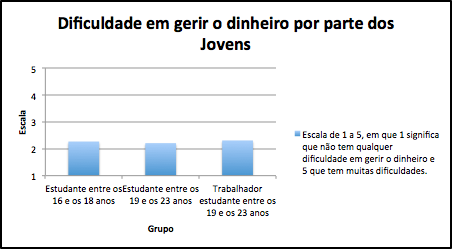
\includegraphics[width=0.7\linewidth]{img/img3}
          \caption{Dificuldade em gerir o dinheiro por parte dos jovens}
          \label{img3}
      \end{figure}

      Em seguida foi perguntado aos jovens se estes estariam dispostos a usar uma aplicação que lhes permitisse gerir facilmente o seu dinheiro e obter dinheiro dos pais rapidamente, mesmo que os pais pudessem controlar os gastos dos filhos. Uma monitorização por parte dos pais é muito importante para que estes possam educar os filhos para uma administração racional e ponderada do dinheiro que lhes disponibilizam.

      Quer a maior parte dos estudantes entre os 16 e os 18 e dos estudantes entre os 19 e 23 revelaram que a sua utilização da aplicação dependeria do controlo por parte dos pais. Já metade dos trabalhadores estudantes, entre os 19 e os 23, estariam dispostos a utilizar a aplicação, apesar do controlo parental.

      \begin{figure}[ht!]
        \centering
          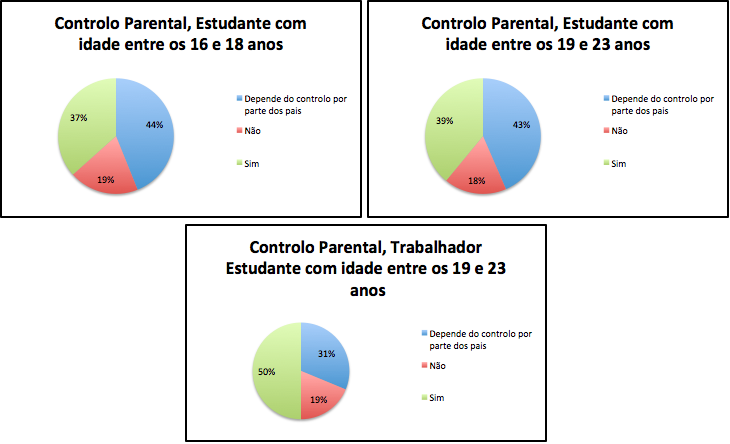
\includegraphics[width=0.7\linewidth]{img/img4}
          \caption{Controlo Parental}
          \label{img4}
      \end{figure}      

      De facto, estas estatísticas mostram que \textbf{o controlo parental terá de ser pensado para não parecer demasiado intrusivo} para os filhos.

      Em seguida foram apresentadas aos jovens algumas das funcionalidades previstas para a aplicação, dando-lhes a conhecer o controlo que os pais iriam ter sobre os seus gastos (estabelecimento de limites, controlo geográfico, consulta dos movimentos, notificações automáticas) e aquilo que será vantajoso para eles se utilizarem a aplicação (disponibilização de semanadas/mesadas, transferências instantâneas de dinheiro, efetuar pagamentos, definir poupanças). Confrontados com estas possibilidades, perguntamos aos jovens se estariam dispostos a utilizar a yWallet. Em todos os grupos as respostas foram superiores a 75\%, destacando-se o grupo dos estudantes entre os 16 e os 18 anos, com 80,49\% de respostas afirmativas, mostrando que \textbf{os mais novos são o grupo mais recetivo à utilização da aplicação}.

      \begin{figure}[ht!]
        \centering
          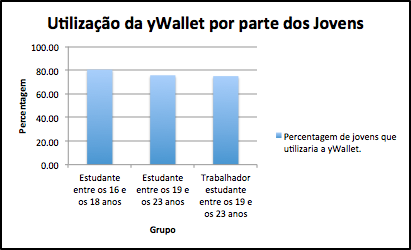
\includegraphics[width=0.7\linewidth]{img/img5}
          \caption{Utilização da yWallet por parte dos jovens}
          \label{img5}
      \end{figure} 

      Seguidamente os inquiridos foram confrontados com um conjunto de funcionalidades, ao qual tiveram de atribuir classificações, de 1 a 5, com o intuito de podermos determinar quais são de facto as funcionalidades mais importantes para os jovens.

      Para os jovens \textbf{estudantes dos 16 aos 18 (P1)}, as três funcionalidades mais importantes são:

      \begin{enumerate}
        \item pôr dinheiro de parte para o poupar para um determinado objetivo;
        \item a aplicação dar conselhos sobre o uso do dinheiro;
        \item obter rapidamente dinheiro dos pais.
      \end{enumerate}

      Para os jovens \textbf{estudantes dos 19 aos 23 (P2)}, as três funcionalidades mais importantes, são:

      \begin{enumerate}
        \item pôr dinheiro de parte para o poupar para um determinado objetivo;
        \item obter rapidamente dinheiro dos pais.
        \item permitir ver com detalhe como o dinheiro é usado.
      \end{enumerate}

      Por fim, para os jovens trabalhadores \textbf{estudantes dos 19 aos 23 (P3)}, as três funcionalidades a que atribuem mais importância são:

      \begin{enumerate}
        \item pôr dinheiro de parte para o poupar para um determinado objetivo;
        \item a aplicação dar conselhos sobre o uso do dinheiro;
        \item permitir ver com detalhe como o dinheiro é usado.
      \end{enumerate}

      As três \textbf{funcionalidades que reúnem mais consenso}, entre os três grupos, no que diz respeito à importância são:

      \begin{enumerate}
        \item pôr dinheiro de parte para o poupar para um determinado objetivo;
        \item a aplicação dar conselhos sobre o uso do dinheiro;
        \item permitir ver com detalhe como o dinheiro é usado.
      \end{enumerate}

      Apresentam-se os dados estatísticos em seguida, em que as funcionalidades encontram-se ordenadas da mais importante para a menos importante.


      \begin{figure}[ht!]
        \centering
          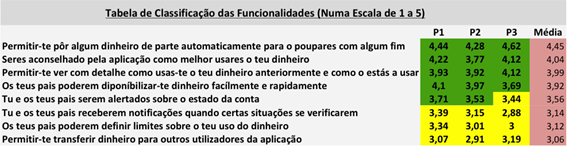
\includegraphics[width=0.7\linewidth]{img/img6}
          \caption{Tabela de classificação das funcionalidades}
          \label{img6}
      \end{figure} 

      Depois de termos dado uma ideia da aplicação que vamos desenvolver, e de todas as funcionalidades que esta oferece, em jeito de conclusão pedimos aos jovens para classificar, de uma forma geral, a yWallet.

      \begin{figure}[ht!]
        \centering
          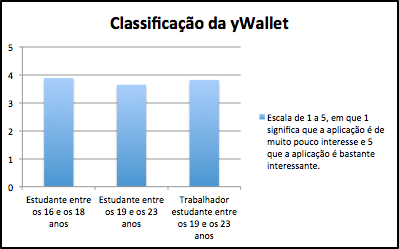
\includegraphics[width=0.7\linewidth]{img/img7}
          \caption{Classificação da yWallet}
          \label{img7}
      \end{figure} 
     
      Os dados obtidos mostram que os inquiridos ficaram efetivamente interessados na aplicação.

    \subsubsection{Questionário dos Pais}

      Para efetuarmos a análise do questionário que remetemos aos pais, selecionamos os três grupos com o maior número de respostas: pais com idades compreendidas entre os 31 e os 35 anos, pais entre os 40 e 50 anos e por último pais com mais de 50 anos. De notar que, 93\% dos pais entre 40 e 50 anos e que 79\% dos pais com mais de 50 anos, são trabalhadores por contra de outrem.

      Todos os inquiridos afirmaram utilizar tecnologias como o tablet, o smartphone ou o computador diariamente.

      Em seguida foi perguntado aos pais se controlam de alguma maneira o dinheiro dos filhos sendo que a grande maioria dos pais entre os 31 e 35 anos dizem não controlar o dinheiro dos filhos (67\%). Por outro lado 1 em cada 2 pais com idades compreendidas entre os 40 e os 50 anos dizem controlar frequentemente o dinheiro dos filhos.

      \begin{figure}[ht!]
        \centering
          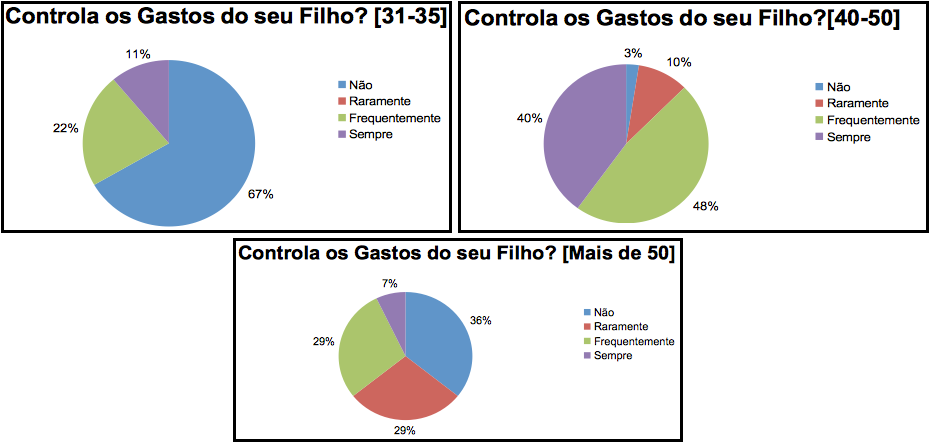
\includegraphics[width=0.7\linewidth]{img/img8}
          \caption{Controlo de gastos dos filhos}
          \label{img8}
      \end{figure}       

      Foi então perguntado aos pais, depois de saber que alguns deles controlam o dinheiro dos filhos frequentemente, se acham dificil executar essa tarefa de controlo do dinheiro. Nas várias faixas etárias, a percentagem de pais que tem dificuldade em controlar o dinheiro dos filhos varia entre 20 e 40\%. Faria então sentido, ter um único sitio em que os pais pudessem ter efectivamente controlo sobre o dinheiro dos filhos? Quanto aos pais com idades superiores aos 40 anos, em média um em cada dois diz que seria de facto útil ter um único sitio onde pudesse controlar os gastos/dinheiro do filho enquanto que esta percentagem é de 89\% no que diz respeito aos pais entre os 31 e 35 anos.

      \begin{figure}[ht!]
        \centering
          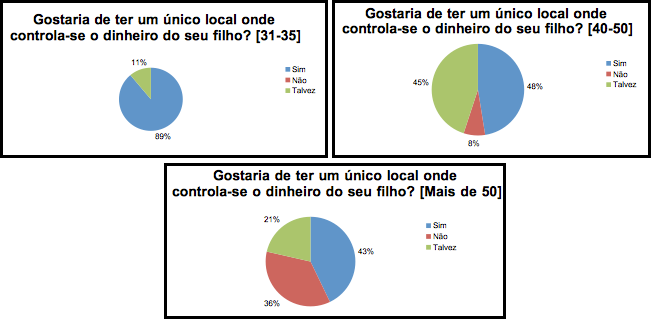
\includegraphics[width=0.7\linewidth]{img/img9}
          \caption{``Gostaria de ter um único local onde controlasse o dinheiro do seu filho''?}
          \label{img9}
      \end{figure}

      Podemos ainda ver no gráfico abaixo em que idades dos filhos é que os pais estariam mais dispostos a utilizar uma aplicação de controlo/gestão de dinheiro. Os resultados mostram que para os pais uma aplicação deste género faria mais sentido nas faixas etárias entre os 11-15 anos e 16-18 anos. 

      \begin{figure}[ht!]
        \centering
          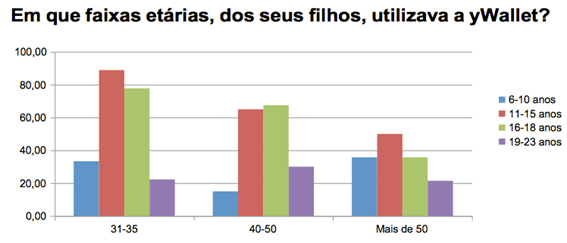
\includegraphics[width=0.7\linewidth]{img/img10}
          \caption{Faixas etárias em que utilizaria a yWallet}
          \label{img10}
      \end{figure}

      Foi então explicado aos pais muito resumidamente que a yWallet seria uma aplicação mobile que os ajudaria a gerir o dinheiro dado por eles aos filhos assim como controlar as suas despesas. Foi-lhes explicado que poderiam, por exemplo, aplicar limites ao dinheiro gasto pelos seus filhos e definir que notificações desejariam receber sobre os gastos dos mesmos; disponibilizar semanadas/mesadas aos seus filhos, bem como transferir/ disponibilizar dinheiro de forma instantânea sem qualquer custo ou ainda restringir os locais onde é possível realizar pagamentos por parte dos seus filhos. 

      Tendo sido isto explicado aos pais foi-lhes perguntado se utilizariam tal aplicação e se pagariam por ela. Todos os pais entre os 31-35 anos disseram que utilizariam a yWallet. Aproximadamente 60\% dos pais entre os 40-50 anos utilizariam a yWallet sendo que apenas 40\% dos pais com mais de 50 anos responderam positivamente a esta pergunta. Quanto a pagar pela aplicação, podemos ver pelos resultados que só alguns pais o fariam. Sendo assim a aplicação deve seguir um modelo \emph{free} com possíveis \emph{upgrades} disponíveis mediante pagamento.

      \begin{figure}[ht!]
        \centering
          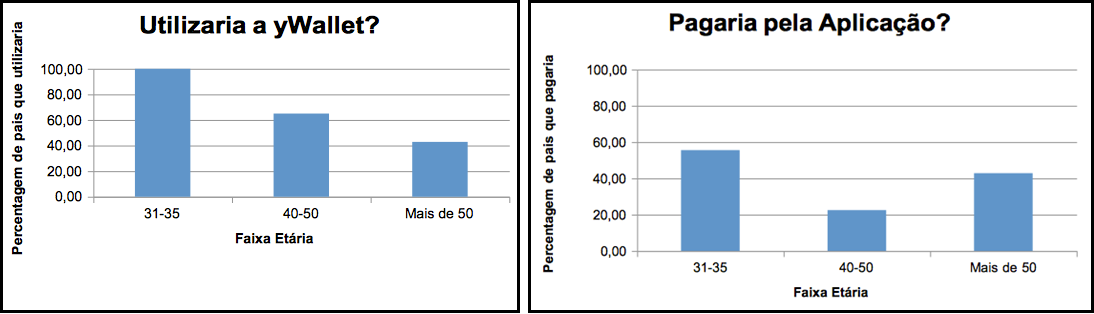
\includegraphics[width=0.7\linewidth]{img/img11}
          \caption{Utilizadores que utilizariam a aplicação}
          \label{img11}
      \end{figure}

      Seguidamente os inquiridos foram confrontados com um conjunto de funcionalidades, ao qual tiveram de atribuir classificações, de 1 a 5, com o intuito de podermos determinar quais são de facto as funcionalidades mais importantes para os pais.

      Para os pais \textbf{com idades entre os 31 e os 35 anos}, as três funcionalidades mais importantes são:

      \begin{enumerate}
        \item Ser alertado sobre o estado da conta;
        \item Controlar os gastos dos seus filhos;
        \item Restringir o pagamento de serviços com base na localização dos seus filhos.
      \end{enumerate} 

      Para os pais \textbf{com idades entre os 40 e os 50 anos}, as três funcionalidades mais importantes são:

      \begin{enumerate}
        \item Ser alertado sobre o estado da conta;
        \item Controlar os gastos dos seus filhos;
        \item Receber notificações e definir em que circunstâncias as quer receber.
      \end{enumerate} 

      Para os pais \textbf{com mais de 50 anos}, as três funcionalidades mais importantes são:

      \begin{enumerate}
        \item Receber notificações e definir em que circunstâncias as quer receber;
        \item Ser alertado sobre o estado da conta;
        \item Controlar os gastos dos seus filhos;
      \end{enumerate}

      Em seguida, apresentam-se os dados estatísticos encontrando-se as funcionalidades ordenadas da mais importante para a menos importante.

      \begin{figure}[ht!]
        \centering
          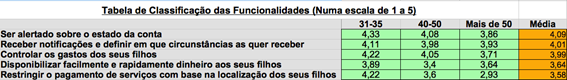
\includegraphics[width=0.7\linewidth]{img/img12}
          \caption{Tabela de Classificação de Funcionalidades}
          \label{img12}
      \end{figure}

      Depois de termos dado uma ideia da aplicação que vamos desenvolver, e de todas as funcionalidades que esta oferece, em jeito de conclusão pedimos aos pais para classificar, de uma forma geral, a yWallet. 

      \begin{figure}[ht!]
        \centering
          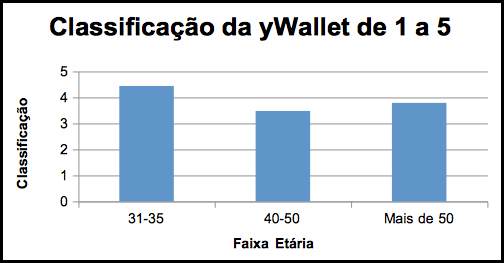
\includegraphics[width=0.7\linewidth]{img/img13}
          \caption{Classificação da yWallet}
          \label{img13}
      \end{figure}

  \subsection{Personas}

    Para melhor identificarmos e representarmos os diferentes tipos de utilizadores da nossa aplicação, definimos algumas personas, de acordo com a informação obtida nas entrevistas e nos questionários:

    \begin{enumerate}
      \item \emph{Filipe Costa, estudante do ensino secundário}\\
            Tem 16 anos de idade e frequenta o 11º ano. Tem um percurso académico razoável, sem reprovações, e tem como objetivo ingressar no curso superior de Licenciatura em Engenharia Informática.

            O Filipe já começa a ter as suas despesas pessoais (alimentação, hobbies, etc.), de modo que os pais lhe dão, todos os meses, uma quantia fixa de dinheiro (mesada). Esta quantia deve ser gerida de tal forma a que o Filipe consiga pagar as suas despesas mais importantes, como a alimentação, e consiga poupar dinheiro para os seus hobbies. É um amante das tecnologias e sempre que consegue poupar dinheiro suficiente, da mesada que os pais lhe dão, gasta-o em novidades tecnológicas.

            Filipe gere o seu dinheiro com recurso a folhas de cálculo mas por vezes esquece-se de apontar as suas despesas, o que implica que no final do mês verifica que tem menos dinheiro do que deveria ter. O maior problema que o Filipe enfrenta é no final do mês verificar que gastou uma quantia elevada de dinheiro em artigos fúteis.

            Por vezes, os pais de Filipe Costa ausentam-se do país em viagens de negócios, o que dificulta, nestes períodos, o acesso a dinheiro extra (quando é necessário) por parte do Filipe.

      \item \emph{Catarina Barbosa, estudante universitária}\\
            Tem 21 anos de idade e frequenta o 3º e último ano da Licenciatura em Psicologia. Esta estudante, ainda dependente dos pais, vive fora da residência dos pais durante o período de aulas. Para facilitar o pagamento das despesas durante o período de aulas, os pais dão uma mesada à Catarina para as despesas mensais.

            Mas por vezes existem despesas não previstas, como por exemplo a compra de livros. Devido ao esforço que os pais fazem para a Catarina poder frequentar a Universidade, ela tenta ao máximo não desperdiçar dinheiro, ou seja, tenta gerir da melhor forma possível o dinheiro por forma a não ser necessário pedir dinheiro extra aos pais quando surgem despesas não previstas.

            Como a Catarina tem um irmão com 15 anos, nem sempre é fácil para os pais da Catarina disponibilizar dinheiro extra à mesada.

      \item \emph{João Cunha, Trabalhador e Estudante Universitário}\\
            Tem 23 anos de idade e é finalista do Mestrado em Design Industrial. O João já tem o seu emprego, ou seja, já não depende do dinheiro dos pais para pagar as suas despesas. No entanto, a vida de trabalhador-estudante não é fácil e o curso do João necessita de bastante material de desenho, por vezes material de valor elevado. Todos os meses é necessário a compra de materiais novos.

            João tem duas irmãs a estudarem na Universidade, o que implica que o João não pode contar com a ajuda dos pais para as suas despesas.

            É necessário que o João saiba gerir o seu ordenado por forma a que consiga pagar todas as suas despesas.

            Como é um jovem estudante, está diariamente em contacto com as tecnologias. Recentemente adquiriu o seu smartphone para poder fotografar os seus trabalhos e enviá-los por e-mail facilmente.

      \item \emph{Miguel Faria, Programador Web}\\
            Tem 34 anos de idade, é casado e tem um filho de 12 anos. O seu filho, Jorge Faria, começa a querer sair com os amigos e a ter as suas próprias coisas.

            Miguel acha que está na altura de ensinar o filho a importância do dinheiro. Mas como Jorge não sabe o que custa a ganhar o dinheiro, Miguel tem receio que o seu filho gaste o dinheiro em coisas fúteis ou perigosas, como o tabaco.

            Miguel não quer ser muito controlador mas quer ter algum controlo sobre a utilização do dinheiro por parte do filho nestes primeiros passos. E ter a certeza que o filho não se mete em vícios que o prejudicam.

            Como Jorge ainda está a dar os primeiros passos em saber como gerir o seu dinheiro, Miguel apenas lhe fornece quantias pequenas, o que implica que o Jorge peça dinheiro ao pai com alguma frequência.

      \item \emph{Rodrigo Pontes, Enfermeiro}\\
            Tem 48 anos de idade, é casado e tem três filhos: o Filipe, com 22 anos, a Carlota com 19 anos e a Margarida com 15 anos. O Filipe e a Carlota são jovens universitários que não residem com os pais no período de aulas. A Margarida é estudante do ensino secundário.

            Para o Rodrigo é bastante importante ter uma forma de gerir o dinheiro de forma fácil que fornece aos seus filhos para que nada falte aos filhos. No entanto, nem sempre é fácil fazer a gestão, pois tem três filhos e dois deles vivem fora de casa em período de aulas.

            Rodrigo tenta ser o mais justo possível com os seus filhos. O que um tem, os outros também têm. Esta justiça é possível através de uma boa gestão das despesas dos filhos.

      \item \emph{Mariana Costa, Advogada}\\
            Tem 55 anos de idade, é divorciada e tem um filho de 20 anos, o Guilherme. Guilherme é um jovem universitário que estuda fora do seu país. Apenas vem a casa duas vezes por ano, no mês de Agosto e no Natal.

            As despesas da Universidade são pagas pelo pai de Guilherme e as despesas do quotidiano, como a alimentação, são pagas pela mãe.

            Sendo assim Guilherme recebe dinheiro do pai e da mãe.

            Mariana verifica todos os meses se o pai de Guilherme transferiu o dinheiro para o seu filho, e dependendo do que sobra dessa quantia após pagar as despesas da universidade, ela transfere o dinheiro necessário para as despesas do quotidiano.

            Devido a Guilherme estudar fora do país, quando surge despesas não previstas é complicado para Mariana disponibilizar dinheiro para o seu filho em tempo útil.

    \end{enumerate}

  \subsection{Requisitos Funcionais e de Dados}

    Os requisitos funcionais descrevem o conjunto de funcionalidades que a nossa solução deverá apresentar, e são orientados às ações que os utilizadores poderão executar.

    A técnica de priorização empregue na atribuição de prioridades aos requisitos funcionais foi a priorização MoSCoW, em que são utilizadas as letras M, S, C e W, que significam, respetivamente, Must have, Should have, Could have, Won’t have. Esta priorização teve em consideração a entrega final do projeto, ou seja: Must have são os requisitos críticos para o sucesso do projeto no contexto da UCE, que têm obrigatoriamente de ser cumpridos; Should have são requisitos importantes; Could have são requisitos menos importantes, que apesar de tudo seriam uma boa adição; Won’t have são requisitos que não são apropriados para o contexto da deadline, mas que serão incluídos caso o projeto tenha continuidade.

    \subsubsection{Uso Geral da Plataforma}

      \begin{description}
        \item[Número:]1
        \item[Descrição:] Um pai e um ou mais filhos criam uma conta no serviço para usarem juntos.
        \item[Fundamentação:] Os pais ao subscrever o serviço criam uma conta juntamente com os seus filhos. Cada conta está associada a um pai e a um ou mais filhos, pois não faz sentido existir um sem o outro no contexto da aplicação.
        \item[Origem:]Equipa do projeto.
        \item[Critério de validação:]Os pais e os filhos conseguem registar-se, e as suas contas ficam disponíveis no sistema.
        \item[Prioridade:]M
      \end{description}
      \vspace{0.5cm}
      \begin{description}
        \item[Número:]2
        \item[Descrição:] Os pais e os filhos podem editar os seus perfis.
        \item[Fundamentação:]Ao ter uma conta têm de ter a possibilidade de atualizar todos os seus dados, caso deixe de utilizar e-mail que utilizou para o registo, ou quaisquer outros dados que a sua conta possua.
        \item[Origem:]Equipa do projeto.
        \item[Critério de validação:]Os dados são alterados e ficam registados na base de dados.
        \item[Prioridade:]M
      \end{description}
      \vspace{0.5cm}
      \begin{description}
        \item[Número:]3
        \item[Descrição:]Os pais autorizam o acesso a uma conta pré-existente de um serviço compatível, que servirá como repositório do dinheiro utilizado pelo nosso serviço.
        \item[Fundamentação:] Para ser possível usar efetivamente dinheiro, é necessário ter uma conta para o conter. Para poder utilizar as funcionalidades que necessitamos, vamos usar um serviço externo ainda a determinar. Para facilitar o processo de depósito de dinheiro, exigimos que a conta seja pré-existente, e que os utilizadores depositem o dinheiro diretamente nesse serviço. 
        \item[Origem:] Equipa do projeto.
        \item[Critério de validação:]A nossa plataforma passa a ter acesso à conta dos utilizadores.
        \item[Prioridade:]M
      \end{description}


    \subsubsection{Restrições de Uso de Dinheiro}  

      \begin{description}
        \item[Número:]4
        \item[Descrição:]Os pais e os filhos podem restringir o uso do dinheiro definindo limites intermédios e máximos, referentes a intervalos de tempo especificáveis (por exemplo, não permitir o uso de mais do que 30\EUR{} durante o período de uma semana). 
        \item[Fundamentação:]Para evitar o mau uso do dinheiro, e garantir que este esteja disponível quando for efetivamente necessário, deve ser possível definir estes limites. As configurações dos pais têm precedência sobre as dos filhos.
        \item[Origem:]Equipa do projeto.
        \item[Critério de validação:]Os filhos apenas podem usar os montantes pré-definidos.
        \item[Prioridade:]M
      \end{description}
\vspace{0.5cm}
      \begin{description}
        \item[Número:]5
        \item[Descrição:]Os pais e os filhos podem restringir o uso do dinheiro com base na localização no momento de compra.
        \item[Fundamentação:]Os pais podem querer que o dinheiro apenas seja usado em lugares específicos, para evitar o mau uso do seu dinheiro, proteger e educar os seus filhos. Os próprios filhos podem também ter essa iniciativa. As configurações dos pais têm precedência sobre as dos filhos.
        \item[Origem:]Equipa do projeto.
        \item[Critério de validação:]Os filhos apenas podem usar o seu dinheiro nas localizações autorizadas.
        \item[Prioridade:]C
      \end{description}


    \subsubsection{Consulta de Informação}

            \begin{description}
        \item[Número:]6
        \item[Descrição:]Os pais e os filhos podem ver os detalhes dos movimentos de conta.
        \item[Fundamentação:]Ser possível rever os movimentos de conta é crítico, que para os pais poderem refletir sobre os hábitos dos filhos, quer para os filhos terem consciência do uso que têm feito do seu dinheiro.
        \item[Origem:]Equipa do projeto.
        \item[Critério de validação:]O histórico dos gastos dos filhos são apresentados aos mesmos/respetivos pais.
        \item[Prioridade:]M
      \end{description}
\vspace{0.5cm}

            \begin{description}
        \item[Número:]7
        \item[Descrição:]Os pais e os filhos podem filtrar os movimentos de conta por intervalo de tempo. 
        \item[Fundamentação:]Deve ser possível ver em detalhe o que ocorreu num intervalo de tempo específico, para facilitar essa análise.
        \item[Origem:]Equipa do projeto.
        \item[Critério de validação:] Os movimentos de conta são apresentados aos pais e aos filhos, filtrados pelo intervalo de tempo especificado.
        \item[Prioridade:]M
      \end{description}
\vspace{0.5cm}

            \begin{description}
        \item[Número:]8
        \item[Descrição:]Os pais e os filhos podem estudar os movimentos de conta conforme a localização onde estes ocorreram. 
        \item[Fundamentação:]A informação de geolocalização é útil e pertinente para a educação do filho.
        \item[Origem:]Equipa do projeto.
        \item[Critério de validação:]Os movimentos de conta são apresentados aos pais e aos filhos, com referência da localização onde ocorreram.
        \item[Prioridade:]C
      \end{description}
\vspace{0.5cm}

            \begin{description}
        \item[Número:]9
        \item[Descrição:]Os pais e os filhos podem ver o estado atual da conta (nomeadamente o seu saldo).
        \item[Fundamentação:]É fulcral poder ver o estado da conta, quer para o pai poder disponibilizar o dinheiro ao filho quando necessário, quer para o filho saber quanto dinheiro pode gastar.
        \item[Origem:]Equipa do projeto.
        \item[Critério de validação:]O estado da conta é apresentado aos mesmos/respetivos pais.
        \item[Prioridade:]M
      \end{description}

    \subsubsection{Notificações}  

            \begin{description}
        \item[Número:]10
        \item[Descrição:]Os pais e os filhos podem especificar quando querem ser notificados, e consequentemente serão notificados quando essas condições se verificarem.
        \item[Fundamentação:]Os pais podem querer receber notificações quando certas situações se verificarem, para poderem agir de acordo. Dependendo do grau de controlo que deseje, estes podem especificar de forma mais ou menos detalhada quando desejam ser notificados.
        \item[Origem:]Equipa do projeto.
        \item[Critério de validação:]Os pais e os filhos recebem notificações quando ocorrem situações em que se verificam as regras definidas por eles para despoletar essas notificações.
        \item[Prioridade:]S
      \end{description}
\vspace{0.5cm}
     \begin{description}
        \item[Número:]11
        \item[Descrição:]Os pais são alertados quando certas situações especiais ocorrem.
        \item[Fundamentação:]Quando certas situações mais comuns e potencialmente mais importantes ocorrem, como por exemplo, quando o saldo na conta do seu filho é insuficiente para uma compra, os pais são notificados.
        \item[Origem:]Equipa do projeto.
        \item[Critério de validação:]Os pais recebem alertas quando essas situações especiais ocorrem.
        \item[Prioridade:]S
      \end{description}

    \subsubsection{Transferência de Dinheiro}  

      \begin{description}
        \item[Número:]12
        \item[Descrição:]Os pais podem autorizar o uso de uma determinada quantia para uma situação pontual.
        \item[Fundamentação:]Quando se sabe previamente que um filho vai ter que fazer uma compra pontual, o pai pode autorizar o uso de um quantia apropriado para essa compra.
        \item[Origem:]Equipa do projeto.
        \item[Critério de validação:]O pai autoriza o uso de uma quantia pré-determinada, e ela fica disponível para ser utilizada pelo filho.
        \item[Prioridade:]S
      \end{description}
\vspace{0.5cm}
      \begin{description}
        \item[Número:]13
        \item[Descrição:]Os pais podem receber pedidos de autorização ao acesso a uma determinada quantia adicional por parte dos filhos, e consequentemente aceitar ou recusar esse pedido.
        \item[Fundamentação:]Para situações excecionais (incluindo situações de emergência) os pais devem poder receber este pedidos parte dos filhos, para estes terem dinheiro disponível quando precisam.
        \item[Origem:]Equipa do projeto.
        \item[Critério de validação:]Os pais são notificados dos pedidos dos filhos, e caso autorizem, os filhos podem usar a quantia que pediram.
        \item[Prioridade:]S
      \end{description}
\vspace{0.5cm}
      \begin{description}
        \item[Número:]14
        \item[Descrição:]Os filhos podem pedir um determinado montante adicional aos pais em situações pontuais.
        \item[Fundamentação:]Em certas situações de emergência, o filho pode não ter dinheiro suficiente para efetuar um pagamento, sendo que deve ser possível que estes consigam, de forma rápida, pedir a quantia que lhes faz falta.
        \item[Origem:]Equipa do projeto.
        \item[Critério de validação:]O pai recebe um pedido de autorização de acesso à quantia de dinheiro que o seu filho especificou.
        \item[Prioridade:]S
      \end{description}

    \subsubsection{Informação}

      \begin{description}
        \item[Número:]15
        \item[Descrição:]Os pais e filhos podem consultar estatísticas relativas à sua conta.
        \item[Fundamentação:]As estatísticas permitirão aos pais e aos filhos consultar hábitos no que diz respeito aos gastos (por mês ou por semana), poupanças (montantes arrecadados), entre outros.
        \item[Origem:]Equipa do projeto.
        \item[Critério de validação:] O utilizador visualiza os dados gerados pela aplicação para a situação requerida.
        \item[Prioridade:]M
      \end{description}

    \subsubsection{Outros}

            \begin{description}
        \item[Número:]16
        \item[Descrição:]Os filhos podem efetuar pagamentos.
        \item[Fundamentação:]Os filhos devem ser capazes de efetuar pagamentos através da aplicação, nos estabelecimentos em que tal seja possível.
        \item[Origem:]Equipa do projeto.
        \item[Critério de validação:]O dinheiro é retirado da conta e transferido para o comerciante.
        \item[Prioridade:]M
      \end{description}
\vspace{0.5cm}
            \begin{description}
        \item[Número:]17
        \item[Descrição:]Os filhos podem transferir dinheiro para outros utilizadores.
        \item[Fundamentação:]Os filhos devem ser capazes de transferir dinheiro para outros utilizadores da aplicação, seja para emprestar ou devolver uma certa quantia de dinheiro.
        \item[Origem:]Equipa do projeto.
        \item[Critério de validação:]O dinheiro é retirado da conta e transferido para o outro utilizador.
        \item[Prioridade:]C
      \end{description}
\vspace{0.5cm}
            \begin{description}
        \item[Número:]18
        \item[Descrição:]Os filhos podem definir e agendar uma poupança.
        \item[Fundamentação:]Os filhos podem querer poupar uma determinada quantia de dinheiro, sendo que a aplicação deve permitir definir uma data para essa quantia ser retirada do saldo disponível.
        \item[Origem:]Equipa do projeto.
        \item[Critério de validação:]Na data estabelecida, a quantia é retirada do saldo disponível e é colocada em cativo.
        \item[Prioridade:]C
      \end{description}

  \subsection{Modelo de Domínio}

    Após o levantamento de requisitos, a análise dos dados obtidos, e algumas sessões de \emph{brainstorming} por parte da equipa de desenvolvimento, conseguimos chegar a um modelo de domínio. A figura seguinte ilustra este modelo sob a forma de diagrama.

    Este modelo já prevê estruturas de dados para a automatização de mesadas, notificações aos utilizadores, definição de regras de uso do dinheiro, e geolocalização dos pagamentos.


      \begin{figure}[ht!]
        \centering
          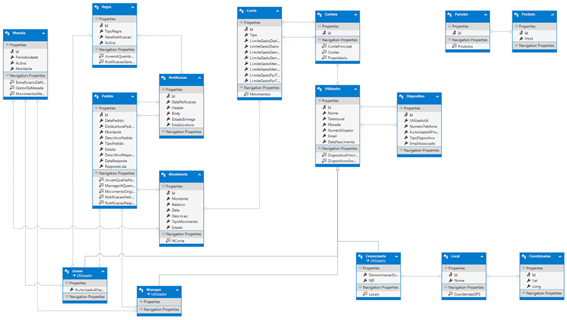
\includegraphics[width=\linewidth]{img/img14}
          \caption{Modelo de Domínio}
          \label{img14}
      \end{figure}

\newpage

\section{Requisitos Não Funcionais}

  Os requisitos não-funcionais são um conjunto de características que um produto deve ter para garantir a sua qualidade.

  Algumas destas características são, por exemplo, a aparência da aplicação, a facilidade de utilização, o desempenho, a segurança que oferece, entre outras.

  O cumprimento do conjunto de normas que se segue será essencial para oferecer um serviço de qualidade aos utilizadores.
  
  A técnica de priorização empregue na atribuição de prioridades aos requisitos não funcionais foi a mesma utilizada para os funcionais - a priorização MoSCoW.

  \subsection{Aparência}

            \begin{description}
        \item[Número:]1
        \item[Descrição:]O produto deve ser atrativo visualmente para todos os utilizadores.
        \item[Fundamentação:]O utilizador deve olhar para o produto e ter vontade de o utilizar. O produto deve ser bem construído de forma a cativar utilizadores de forma fácil e eficaz. 
        \item[Origem:] Equipa do projeto.
        \item[Critério de validação:] Equipa do projeto.
        \item[Prioridade:]S
      \end{description}
      \vspace{0.5cm}
            \begin{description}
        \item[Número:]2
        \item[Descrição:]O produto deve ser construído de forma a que as pessoas se sintam confortáveis e confiem ao utilizar o mesmo. 
        \item[Fundamentação:]O produto deve garantir que os seus utilizadores confiem no mesmo. O produto deve assim ser claro e especificar de forma objetiva tudo aquilo que faz. Deve ter um aspeto profissional.
        \item[Origem:]Equipa do projeto.
        \item[Critério de validação:]A grande maioria dos utilizadores deve sentir-se segura ao utilizar o produto.
        \item[Prioridade:]M
      \end{description}
  \subsection{Usabilidade}
     \begin{description}
        \item[Número:]3
        \item[Descrição:] Os utilizadores devem conseguir aprender a utilizar o produto com facilidade.
        \item[Fundamentação:]Se os utilizadores não conseguirem fazer aquilo que pretendem de uma forma fácil e direta, podem deixar de usar o produto.
        \item[Origem:]Equipa do projeto.
        \item[Critério de validação:]Um utilizador deve ser capaz dominar as funcionalidades que o produto lhe oferece após entrar em contacto com o mesmo pela primeira vez.
        \item[Prioridade:]S
      \end{description}
      \vspace{0.5cm}
      \begin{description}
        \item[Número:]4
        \item[Descrição:]Os utilizadores devem conseguir utilizar o produto independentemente das línguas que conhece e domina.
        \item[Fundamentação:]O produto deve ser capaz de apresentar a informação em diferentes idiomas para assim facilitar a sua utilização.
        \item[Origem:]Equipa do projeto.
        \item[Critério de validação:]O utilizador compreende e percebe o conteúdo apresentado corretamente.    
        \item[Prioridade:]C
      \end{description}
      \vspace{0.5cm}
      \begin{description}
        \item[Número:]5
        \item[Descrição:]Os utilizadores devem conseguir utilizar o produto independentemente da moeda que utiliza no dia a dia.
        \item[Fundamentação:]O produto deve ser capaz de apresentar o valor monetário e trabalhar com diferentes tipos de moedas.
        \item[Origem:]Equipa do projeto.
        \item[Critério de validação:]O utilizador consegue escolher o seu tipo preferido de moeda e utilizá-lo no produto.
        \item[Prioridade:]W
      \end{description}
      \vspace{0.5cm}
      \begin{description}
        \item[Número:]6
        \item[Descrição:]Os utilizadores devem conseguir perceber a linguagem utilizada no produto de forma fácil e clara.
        \item[Fundamentação:]O produto deve ser utilizar uma linguagem direcionada ao publico alvo, sendo esta clara de forma a não gerar dúvidas ao utilizador.
        \item[Origem:]Equipa do projeto.
        \item[Critério de validação:]O utilizador percebe de forma clara a linguagem utilizada pelo produto.
        \item[Prioridade:]S
      \end{description}

  \subsection{Desempenho}

      \begin{description}
        \item[Número:]7
        \item[Descrição:]O tempo médio necessário para carregar as páginas da aplicação web não deve ser superior a 5 segundos, numa ligação de rede normal.
        \item[Fundamentação:]Os utilizadores não gostam de esperar para ter acesso a conteúdos.
        \item[Origem:]Equipa do projeto.
        \item[Critério de validação:]As páginas da aplicação devem demorar em média até 5 segundos a carregar, com uma ligação de largura de banda de 4Mbps.
        \item[Prioridade:]M
      \end{description}
      \vspace{0.5cm}
            \begin{description}
        \item[Número:]8
        \item[Descrição:]A aplicação móvel deve ser fluida em todos os dispositivos móveis suportados.
        \item[Fundamentação:]Os utilizadores gostam que as aplicações processem rapidamente os seus pedidos.
        \item[Origem:]Equipa do projeto.
        \item[Critério de validação:]A aplicação corre de forma fluida num dispositivo com processador de 1 GHz e memória RAM de 512 Mb.
        \item[Prioridade:]M
      \end{description}
      \vspace{0.5cm}
            \begin{description}
        \item[Número:]9
        \item[Descrição:]A aplicação deve estar disponível 99\% do ano.
        \item[Fundamentação:]Os utilizadores devem poder utilizar a aplicação sempre que quiserem.
        \item[Origem:]Equipa do projeto.
        \item[Critério de validação:]O servidor está disponível 99\% do ano.
        \item[Prioridade:]W
      \end{description}
      \vspace{0.5cm}

            \begin{description}
        \item[Número:]10
        \item[Descrição:]Os valores monetários deverão ser precisos até à unidade transacional mais pequena.
        \item[Fundamentação:] Dependendo do tipo de moeda, é necessário utilizar as casas decimais adequadas para que não se perca dinheiro em transações.
        \item[Origem:]Equipa do projeto.
        \item[Critério de validação:]Todas as transações são feitas com precisão.
        \item[Prioridade:]S
      \end{description}
      \vspace{0.5cm}

            \begin{description}
        \item[Número:]11
        \item[Descrição:]Em circunstâncias anormais em que o sistema falhe, este é capaz de recuperar rapidamente.
        \item[Fundamentação:]A arquitetura do sistema deverá incluir mecanismos de tolerância a faltas para combater possíveis falhas de determinados componentes. 
        \item[Origem:]Equipa do projeto.
        \item[Critério de validação:]O tempo de indisponibilidade não excede 5 minutos.
        \item[Prioridade:]C
      \end{description}

  \subsection{Operação}

            \begin{description}
        \item[Número:]12
        \item[Descrição:]O tempo de um pagamento/transferência deve ser inferior a 30 segundos.
        \item[Fundamentação:]Para além de ser determinante para a qualidade do serviço, o tempo que um utilizador está disposto a esperar para que possa efetuar um pagamento/transferência é limitado.
        \item[Origem:]Equipa do projeto.
        \item[Critério de validação:]Os pagamentos/transferências são realizados em menos de 30 segundos.
        \item[Prioridade:]M
      \end{description}
      \vspace{0.5cm}


     \begin{description}
        \item[Número:]13
        \item[Descrição:]Ao efetuar pagamentos/transferências, os utilizadores não podem perder dinheiro.
        \item[Fundamentação:]Caso um utilizador perca dinheiro, a qualidade do serviço é posta em causa.
        \item[Origem:] Equipa do projeto.
        \item[Critério de validação:] Qualquer pagamento/transferência resulta sempre no débito de uma dada quantia de uma conta origem, e no crédito dessa quantia exata na conta destino.
        \item[Prioridade:]M
      \end{description}
      \vspace{0.5cm}

      \begin{description}
        \item[Número:]14
        \item[Descrição:]A aplicação depende da utilização da API de uma wallet digital externa ao serviço.
        \item[Fundamentação:]A aplicação utiliza a API de uma wallet digital para efetuar transações e para converter valores monetários em diferentes tipos de moeda.
        \item[Origem:]Equipa do projeto.
        \item[Critério de validação:]A comunicação entre a aplicação e as APIs que utiliza é sempre bem sucedida.
        \item[Prioridade:]M
      \end{description}

  \subsection{Manutenção, Portabilidade e Suporte}    

      \begin{description}
        \item[Número:]15
        \item[Descrição:]Os erros da aplicação devem poder ser reportados pelos utilizadores.
        \item[Fundamentação:]Quando ocorre um erro na aplicação, deverá ser dada a possibilidade do utilizador comunicar esse erro, para que possa ser resolvido.
        \item[Origem:] Equipa do projeto.
        \item[Critério de validação:]A equipa de desenvolvimento é notificada quando os utilizadores reportam erros.
        \item[Prioridade:]C
      \end{description}
      \vspace{0.5cm}

      \begin{description}
        \item[Número:]16
        \item[Descrição:]Os erros reportados pelos utilizadores têm de ser corrigidos.
        \item[Fundamentação:] Os utilizadores não gostam de utilizar aplicações que apresentem erros e problemas.
        \item[Origem:]Equipa do projeto.
        \item[Critério de validação:]Depois de serem reportados, os erros têm de ser corrigidos num prazo adequado à sua gravidade.
        \item[Prioridade:]W
      \end{description}
      \vspace{0.5cm}

      \begin{description}
        \item[Número:]17
        \item[Descrição:]A aplicação deve disponibilizar um espaço para apoio aos utilizadores.
        \item[Fundamentação:]Os utilizadores têm a necessidade de esclarecer dúvidas, por isso deve ser criado um formulário para pedidos de esclarecimento. Para além disso, terá um menu de ajuda para explicar sucintamente as várias funcionalidades ao utilizador.
        \item[Origem:]Equipa do projeto.
        \item[Critério de validação:]As dúvidas dos utilizadores têm de ser esclarecidas, por e-mail, num prazo de 24 horas.
        \item[Prioridade:]C
      \end{description}
      \vspace{0.5cm}

            \begin{description}
        \item[Número:]18
        \item[Descrição:]O produto deve funcionar corretamente nos diferentes tipos de dispositivos suportados.
        \item[Fundamentação:]O produto deve funcionar em vários tipos de dispositivo móvel (Android, iOS) e ainda em vários browsers (Firefox, Chrome, Safari).
        \item[Origem:]Equipa do projeto.
        \item[Critério de validação:]O produto funciona de forma correta nos dispositivos definidos.
        \item[Prioridade:]M
      \end{description}

  \subsection{Segurança}

            \begin{description}
        \item[Número:]19
        \item[Descrição:]As funcionalidades e os dados a que utilizadores têm acesso estão limitados por definições de direitos de acesso.
        \item[Fundamentação:]Só utilizadores devidamente identificados e autenticados têm acesso à aplicação, e o conjunto de funcionalidades a que um determinado utilizador tem acesso é determinado pelo tipo da sua conta de utilizador.
        \item[Origem:]Equipa do projeto.
        \item[Critério de validação:]Os utilizadores têm conhecimento da política de recolha de dados e aceitam ou recusam a mesma.
        \item[Prioridade:]W
      \end{description}
      \vspace{0.5cm}

            \begin{description}
        \item[Número:]20
        \item[Descrição:]Toda a política de recolha de dados deve ser explícita e clara para todos os utilizadores.
        \item[Fundamentação:]A aplicação só irá recolher informações sobre os utilizadores se estes o permitirem.
        \item[Origem:]Equipa do projeto.
        \item[Critério de validação:]Os utilizadores têm conhecimento da política de recolha de dados e aceitam ou recusam a mesma.
        \item[Prioridade:]W
      \end{description}
      \vspace{0.5cm}

            \begin{description}
        \item[Número:]21
        \item[Descrição:]Qualquer alteração na política de informação deve ser informada aos utilizadores. 
        \item[Fundamentação:]O utilizador tem que estar sempre devidamente informado de tudo o que diz respeito às políticas utilizadas pela equipa do produto. Sempre que alguma alteração é feita deve ser imediatamente comunicada aos utilizadores.
        \item[Origem:] Equipa do projeto.
        \item[Critério de validação:]Os utilizadores são notificados das alterações.
        \item[Prioridade:]W
      \end{description}
      \vspace{0.5cm}

            \begin{description}
        \item[Número:]22
        \item[Descrição:]A aplicação deve impedir a introdução de input malicioso.
        \item[Fundamentação:]Devem ser utilizadas técnicas de programação segura que impeçam os atacantes de explorar vulnerabilidades através de injeção de código.
        \item[Origem:]Equipa do projeto.
        \item[Critério de validação:]Os utilizadores não conseguem injetar código na aplicação.
        \item[Prioridade:]M
      \end{description}

      \vspace{0.5cm}

            \begin{description}
        \item[Número:]23
        \item[Descrição:]A aplicação não deve relevar informações que comprometam o seu funcionamento.
        \item[Fundamentação:]No caso de ocorrência de erros, o output produzido não deve revelar  quaisquer informações sobre a implementação, caso contrário atacantes podem aproveitar essas situações para estudar possíveis vulnerabilidades.
        \item[Origem:]Equipa do projeto.
        \item[Critério de validação:]Os utilizadores não conseguem obter informações sobre a implementação.
        \item[Prioridade:]S
      \end{description}
      \vspace{0.5cm}

            \begin{description}
        \item[Número:]24
        \item[Descrição:]A aplicação deve garantir autenticidade, confidencialidade e integridade na ligação ao servidor central.
        \item[Fundamentação:]Uma vez que utilizadores mal intencionados podem observar e manipular as informações que circulam no canal de comunicação entre os utilizadores e o servidor, este deve ser devidamente protegido.
        \item[Origem:] Equipa do projeto.
        \item[Critério de validação:]A aplicação utiliza um protocolo da segurança para proteger as comunicações.
        \item[Prioridade:]M
      \end{description}

  \subsection{Culturais e Políticos}

            \begin{description}
        \item[Número:]25
        \item[Descrição:]A aplicação não deve ser ofensiva para grupos religiosos ou étnicos.
        \item[Fundamentação:]Qualquer tipo de conteúdo sobre grupos religiosos ou étnicos na aplicação deve ser evitado ou bastante ponderado, visto que pode ofender esses mesmos grupos, pondo em risco a imagem da aplicação e mesmo a sua utilização.
        \item[Origem:]Equipa do projeto.
        \item[Critério de validação:]Os conteúdos da aplicação são revistos.
        \item[Prioridade:]W
      \end{description}
      \vspace{0.5cm}

            \begin{description}
        \item[Número:]26
        \item[Descrição:]A aplicação deverá conseguir distinguir vários sistemas numéricos.
        \item[Fundamentação:]Visto que existem sistemas númericos em que se usam pontos em vez de vírgulas para separar as casas decimais, a aplicação deverá estar preparada para processar o input independentemente do sistema númerico utilizado.
        \item[Origem:]Equipa do projeto.
        \item[Critério de validação:]A aplicação processa corretamente o input independentemente do sistema númerico utilizado.
        \item[Prioridade:]C
      \end{description}

  \subsection{Legais}

            \begin{description}
        \item[Número:]27
        \item[Descrição:] A aplicação é compatível com legislação relativa à proteção de dados.
        \item[Fundamentação:]A informação pessoal dos utilizadores armazenada pela aplicação tem de cumprir a legislação.
        \item[Origem:]Equipa do projeto.
        \item[Critério de validação:]A aplicação está de acordo com a legislação.
        \item[Prioridade:]W
      \end{description}
\newpage

\section{Problemas do Projeto}
  
  \subsection{Produtos Reutilizáveis}

  Em qualquer projeto é essencial averiguar o que o mercado oferece para reutilização. A reutilização de componentes evita esforço desnecessário, e promove mais tempo de foco no objetivo principal. Este projeto irá utilizar produtos e bibliotecas existentes para assegurar segurança, robustez e interoperabilidade das aplicações a desenvolver. Estes recursos serão utilizados para fins como a construção da interface com o utilizador nas diversas plataformas, e a geração da documentação da API REST que será desenvolvida.

  \begin{enumerate}
   \item \emph{Phonegap}\\
          O produto deve ser desenvolvido num conjunto de tecnologias, baseadas em standards web, e correr nativamente em cada um dos dispositivos, para minimizar o custo de desenvolvimento, e garantir o acesso a funcionalidades nativas de cada dispositivo.
   \item \emph{Swagger}\\
          Este produto facilita a geração automática da documentação para a API REST a desenvolver.
  \end{enumerate}

  \subsection{Tarefas}

    O projeto será realizado utilizando uma metodologia Scrum. Cada funcionalidade da aplicação será desenvolvida na sua totalidade uma de cada vez, e o trabalho será particionado em pequenas tarefas rápidas. Serão também feitas discussões diárias do estado do projeto através de ferramentas de comunicação, como o Slack.

    O projeto terá as seguintes fases, que terão a duração média indicada:

\paragraph{}
    \textbf{} \\
    2 semanas --- Construção do modelo de domínio, do diagrama de use cases e do diagrama de classes; Design da interface gráfica da aplicação.
\paragraph{}
    \textbf{}\\
    2 semanas --- Implementação dos requisitos MUST.
\paragraph{}
    \textbf{}\\
    2 semanas --- Implementação dos requisitos SHOULD.
\paragraph{}
    \textbf{}\\
    1 semana --- Implementação dos requisitos COULD. Caso as duas fases anteriores demorarem mais que o previsto, o número de requisitos implementados nesta fase será reduzido.
\paragraph{}
    \textbf{}\\
    1 semana --- Realização de testes de desempenho.
\paragraph{}
    \textbf{}\\
    2 semanas --- Criação da documentação necessária.

    \begin{enumerate}
      \item \textbf{Modelação} \hfill
        \begin{description}
          \item[2 semanas] --- Construção do modelo de domínio, do diagrama de use cases e do diagrama de classes; Design da interface gráfica da aplicação.
        \end{description}
      \item \textbf{Implementação Milestone 1}\hfill
        \begin{description}
          \item[2 semanas] --- Implementação dos requisitos MUST.
        \end{description}
      \item \textbf{Implementação Milestone 2}\hfill
        \begin{description}
          \item[2 semanas] --- Implementação dos requisitos SHOULD.
        \end{description}
      \item \textbf{Implementação Milestone 3}\hfill
        \begin{description}
          \item[1 semana] --- Implementação dos requisitos COULD. Caso as duas fases anteriores demorarem mais que o previsto, o número de requisitos implementados nesta fase será reduzido.
        \end{description}
      \item \textbf{Testes}\hfill
        \begin{description}
          \item[1 semana] --- Realização de testes de desempenho.
        \end{description}
      \item \textbf{Documentação}\hfill
        \begin{description}
          \item[2 semanas] --- Criação da documentação necessária.
        \end{description}
          
    \end{enumerate}

  \subsection{Riscos}

    Qualquer projeto, ou negócio, tem riscos associados, pelo menos em alguma fase do seu ciclo de vida. Em particular, há riscos típicos de um projeto de software em métodos eletrónicos de pagamento, conforme identificado nesta secção.

    \begin{enumerate}
      \item \emph{Incumprimento das deadlines.}\\
O primeiro risco associado a qualquer projeto, será sempre o incumprimento dos prazos estipulados para este, ou mesmo a não concretização do projeto. Este risco poderá concretizar-se por fatores como fraca produtividade, má organização entre a equipa, insuficiência de tempo para a dimensão dos objetivos, ou mesmo por uma junção destes fatores. Neste caso, implicará um produto com uma implementação parcial.
      \item \emph{Má adoção do produto.}\\
É possível que o produto não tenha a adesão esperada, quer por parte dos jovens, quer por parte dos pais. Isto poderá dever-se a uma fraca divulgação, insuficientes demonstrações ou métodos de experimentação por parte dos utilizadores, ou mesmo um receio por parte dos utilizadores em adotar métodos de pagamento eletrónicos.
      \item \emph{Dificuldades na aceitação do pagamento eletrónico.}\\
Este projeto assenta em tecnologias e meios de pagamento recentes, como o Bitcoin, que ainda não fazem parte do dia-a-dia do mercado geral. Em particular, o Bitcoin tem uma incidência mais forte nos mercados virtuais, como compras online, quando comparado aos mercados físicos. Contudo, o uso de Bitcoin não é o objetivo do projeto, mas sim uma ferramenta, o que não compromete o projeto como um todo, no caso da concretização deste risco. As respostas a este risco poderão passar pela implementação de adicionais métodos de pagamento, ou até parcerias com alguns comerciantes, para estimular a aceitação do Bitcoin.
      \item \emph{Insuficiência de lucros.}\\
      Qualquer projeto corre o risco de não estar assente sobre um modelo de negócio lucrativo, ou adequado ao contexto. Neste caso, existe, por exemplo, um risco de o produto ser bem aceite, mas não haver adesão suficiente à versão premium, reduzindo os ganhos. A resposta geral passa por rever o modelo de negócios. Para o exemplo dado, uma possível resposta passa por criar ou divulgar de forma mais eficaz os incentivos de aderir à versão premium do produto.
    \end{enumerate}

 \subsection{Custos}
    Os custos associados com o projecto estão descritos em pormenor no documento anexo ``Plano de Negócio''.

  \subsection{Documentação}
    A documentação é um componente crucial de qualquer produto, especialmente num produto de software. A facilidade de uso de um produto, ou da sua interface com o utilizador, é um aspeto subjetivo: o que pode ser intuitivo para um utilizador, poderá não ser para o seguinte. E, de uma forma geral, quem testa um produto, antes de este ser oficialmente lançado ao público, já está por dentro do assunto, já conhece o produto de alguma forma, o que facilita o seu entendimento. Contudo, o produto deve ser utilizável por qualquer pessoa, independentemente do seu nível de familiaridade ou experiência. Isto implica que o produto esteja munido de documentação orientada ao utilizador.

    Toda a documentação que acompanha este produto será produzida e mantida pela equipa de desenvolvimento do produto. Segue, no restante desta secção, uma descrição de cada componente da documentação fornecida ao utilizador.

    \subsubsection{Manual de Instalação}
      \begin{description}
        \item[Propósito:]O manual de instalação tem o objetivo de descrever, detalhada e inequivocamente, todos os passos a tomar pelo utilizador para que este possa instalar e usufruir do produto. Este documento deve também incluir quaisquer pré-requisitos exigidos para a instalação ou uso do produto.
        \item[Utilizadores do documento:]Todos. Qualquer utilizador final do produto deverá seguir as instruções descritas neste manual.

        \item[Manutenção do documento:]Iterativa. Novas versões do produto ou ambiguidades do manual deverão exigir uma revisão do documento.
        \item[Formato:]Documento digital.
      \end{description}

    \subsubsection{Manual do Utilizador}
      \begin{description}
        \item[Propósito:]O manual do utilizador é um documento de comunicação técnico com o propósito de dar assistência aos utilizadores do produto, nas diversas situações que poderão decorrer com a sua utilização. Este manual descreve as funcionalidades do produto, contém todas as informações essenciais para um utilizador fazer pleno uso deste, e inclui ainda todas as instruções, passo-a-passo, para o uso do produto e resolução de problemas comuns.
        \item[Utilizadores do documento:]Todos. Qualquer utilizador final do produto poderá recorrer a este manual, quer para uma utilização inicial da aplicação, quer para esclarecimentos posteriores.

        \item[Manutenção do documento:]Iterativa. Novas versões do produto ou ambiguidades do manual deverão exigir uma revisão do documento.

        \item[Formato:]Documento digital.
      \end{description}

    \subsubsection{Guia de Iniciação Rápida}
      \begin{description}
        \item[Propósito:]O guia de iniciação rápida serve como um tutorial para novos utilizadores. É uma versão muito sucinta do manual do utilizador, com uma forte vertente de comunicação através de imagens, que transmite ao utilizador o essencial a saber para começar a utilizar o produto.

        \item[Utilizadores do documento:]Todos. Qualquer novo utilizador deverá dar utilidade a este guia para começar a tirar proveito do produto logo à partida.

        \item[Manutenção do documento:]Iterativa. Novas versões do produto ou ambiguidades do guia deverão exigir uma revisão do documento.
        \item[Formato:]Documento digital, vídeo e/ou tutorial interativo online, na página do produto.
      \end{description}

    \subsubsection{Manual de Procedimentos de Emergência}
      \begin{description}
        \item[Propósito:]O manual de procedimentos de emergência acompanha o utilizador nos passos a seguir, quando alguma situação inesperada surge. Deverá cobrir, detalhadamente, situações como perda de acesso ao produto, falhas de segurança, ou eventuais inconsistências nas transações monetárias.
        \item[Utilizadores do documento:]Todos. Qualquer utilizador do produto está suscetível a uma situação imprevista, e deverá estar informado das ações a tomar.
        \item[Manutenção do documento:]Iterativa. Novas versões do produto ou ambiguidades do manual deverão exigir uma revisão do documento.
        \item[Formato:]Documento digital.
      \end{description}

    \subsubsection{Folheto de Perguntas Frequentes}
      \begin{description}
        \item[Propósito:]O folheto de perguntas frequentes é um documento de conveniência para o utilizador. Não trata informação que não esteja detalhada nos restantes manuais, mas, contudo, sintetiza as perguntas e situações mais frequentes com que os utilizadores se deparam, reduzindo, portanto, o seu tempo de pesquisa por uma solução.
        \item[Utilizadores do documento:]Todos. Qualquer utilizador, em particular os menos familiares com o produto, poderão deparar-se com problemas comuns, para os quais procuram uma resposta rápida.
        \item[Manutenção do documento:]Iterativa. Novas versões do produto, ambiguidades do folheto, ou novos problemas que surjam frequentemente deverão exigir uma revisão do documento.
        \item[Formato:]Documento digital.
      \end{description}

    \subsubsection{Menu de Ajuda}
      \begin{description}
        \item[Propósito:]O produto deverá suportar um menu de ajuda, onde o utilizador possa esclarecer dúvidas frequentes, de forma sucinta. Serve como uma conveniência, para que o utilizador possa superar dificuldades no uso da aplicação sem ter de recorrer aos manuais.

        \item[Utilizadores do documento:]Todos. Qualquer utilizador, em particular os menos familiares com o produto, poderão deparar-se com problemas comuns, para os quais procuram uma resposta rápida.
        \item[Manutenção do documento:]Iterativa. Novas versões do produto, ou novos problemas que surjam frequentemente deverão exigir uma revisão do menu.
        \item[Formato:]Parte integrante do software produzido.
      \end{description}

    \subsubsection{Licença e Termos de Uso do Produto}
      \begin{description}
        \item[Propósito:]Qualquer produto de software deverá estar acompanhado de uma licença de uso. A licença deixa claro para o utilizador quais as suas permissões e as suas responsabilidades com o uso do produto.
        \item[Utilizadores do documento:]Todos. A licença do produto aplica-se a qualquer utilizador do produto.
        \item[Manutenção do documento:]Iterativa. Ambiguidades na licença ou alterações aos termos de uso deverão exigir uma revisão do documento, sobre a qual todos os utilizadores deverão ser notificados.
        \item[Formato:]Documento digital.
      \end{description}

  \subsection{Trabalho Futuro}

    O trabalho futuro neste projeto passa essencialmente por implementar os requisitos com os níveis de prioridade mais baixos, aqueles que consideramos menos substanciais para o contexto da UCE. Estes serão implementados caso o projeto veja continuidade.

    Planeamos, de acordo com a visão do nosso produto, que os utilizadores consigam utilizar o produto independentemente da moeda que utilizam no dia-a-dia, o que fará com que mais pessoas vejam utilidade em usar o produto.

    Devemos criar mecanismos para que os utilizadores possam reportar erros e problemas da aplicação, o que nos permitirá mantê-la melhorá-la.

    Teremos de elaborar uma declaração da política de recolha e tratamento de dados, compatível com a legislação, bem como assegurar que os utilizadores se mantêm informados sobre a mesma.

    E por fim, teremos que estabelecer uma empresa para o desenvolvimento deste produto e criar uma solução final coesa, para que o produto seja lançado no mercado.

    \nocite{*}
    \bibliography{visaoproduto}{}
    \bibliographystyle{plain}

\end{document}


% \begin{table*}[ht]\centering
%     \RowStretch{1.3}
%     \begin{tabular}{@{}lccccccc@{}}\toprule
%     Col1    & Col2  & Col3  & Col4  & Col5  & Col6 \\
%     \midrule
%     Val1    & Val2  & Val3  & Val4  & Val5  & Val6 \\
%     \bottomrule
%     \end{tabular}
%     \caption{A sample table.}
%     \label{tab:label}
% \end{table*}


      \begin{figure}[ht!]
        \centering
          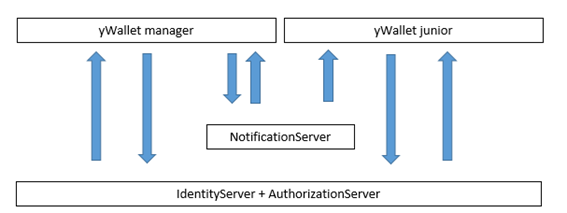
\includegraphics[width=0.7\linewidth]{img/img1}
          \caption{Arquitetura da solução proposta}
          \label{img1}
      \end{figure}